\RequirePackage{ifpdf}
\newif\ifelektroniczna
\newif\ifjednostronna

%\elektronicznatrue
\elektronicznafalse

\jednostronnafalse
% \jednostronnatrue

\ifjednostronna
\def\strony{oneside,openany}
\else
\def\strony{twoside,openright}
\fi

\ifpdf
\documentclass[pdftex,12pt,a4paper,\strony,colorlinks,nocenter,noupper,crosshair]{thesis}
\usepackage[pdftex]{graphicx}
\usepackage[pdftex]{hyperref}
\usepackage[tableposition=top]{caption}
\hypersetup{colorlinks,%
  citecolor=black,%
  filecolor=black,%
  linkcolor=black,%
  urlcolor=black,%
pdftex}
\pdfcompresslevel=1
\else
\documentclass[12pt,a4paper,\strony,nocenter,noupper,crosshair]{thesis}
\usepackage{graphicx}
\fi

\usepackage{wrapfig}
\usepackage{lscape}
\usepackage{rotating}
\usepackage{url}
\usepackage{TitlePage}
\usepackage{theoremref}
\usepackage{mathtools}
\usepackage{tikz}
\usepackage{algorithm}% http://ctan.org/pkg/algorithms
\usepackage{algpseudocode}% http://ctan.org/pkg/algorithmicx
\usepackage{enumerate}
\makeatletter
\renewcommand{\ALG@name}{Pseudokod}
\renewcommand{\listalgorithmname}{Zbiór pseudokodów}
\renewcommand{\algorithmicrequire}{\textbf{Argumenty: }}
\renewcommand{\algorithmicensure}{\textbf{Wynik: }}
\makeatother
\usetikzlibrary{calc, shapes, backgrounds}
\usepackage[utf8]{inputenc}
\def\rodzaj{Praca magisterska}

\def\wydzial{Automatyki, Elektroniki i~Informatyki}

\def\tytul{Parametryzowana złożoność obliczeniowa}
\def\tytulpdf{Parametryzowana złożoność obliczeniowa}

\def\autor{Autor: Korneliusz Adam Caputa}
\def\promotor{Kierujący pracą: prof.~dr~hab.~inż. Zbigniew Czech}
\def\konsultant{}
\def\data{Gliwice, listopad 2014}
\def\slowakluczowe{Fixed point tractability,graph theory,vertex cover,kernelization}

\graphicspath{{./pictures/}}

\DeclareUnicodeCharacter{00A0}{~}

\ifpdf
\ifelektroniczna
\usepackage[
  pdfusetitle=true,
  pdfsubject={\tytulpdf},
  pdfkeywords={\slowakluczowe},
  pdfcreator={\autor},
  pdfstartview=FitV,
  linkcolor=blue,
  citecolor=red,
]{hyperref}
\fi
\fi

\usepackage{layout}

\usepackage{t1enc,amsmath}
\usepackage[OT4,plmath]{polski}
\usepackage{helvet}

%\usepackage{anysize}
%\marginsize{3cm}{2.5cm}{2.5cm}{2.5cm}%LPGD
%\setlength{\textheight}{24cm}
%\usepackage{multirow}
%\ifpdf\usepackage{pdflscape}\else\usepackage{lscape}\fi
%\usepackage{longtable}
%\usepackage{geometry}
%GATHER{thesis.bib}
%\usepackage[twoside]{geometry}
%\geometry{ lmargin=3.5cm, rmargin=2.5cm, tmargin=3cm, bmargin=3cm,
%headheight=1cm, headsep=0.5cm, footskip=0pt }
%\def\fixme#1{}f

\textwidth 150mm
\textheight 225mm
\usepackage{amsfonts}
\usepackage{amsthm}
\usepackage{subfig}
\usepackage{caption}
\captionsetup[subfigure]{justification=centerfirst}
\usepackage{cite}
\usepackage{listings}
\lstset{
  language={Go},
  captionpos=b,
  inputencoding=utf8
}
\usepackage{cleardpempty}
\usepackage{float}
\usepackage{textcomp}
\def\vec#1{\ensuremath{\mathbf{#1}}}
\def\ang#1{ang.~\emph{#1}}
\def\lat#1{lac.~\emph{#1}}
\def\e{\ensuremath{\textrm{\normalfont{}e}}}
\def\degree{\ensuremath{^{\circ}}\protect}
\def\fixme#1{\marginpar{\tiny{}#1}}
\def\labelitemi{--}
\def\labelitemii{--}
\def\labelitemiii{--}

\newtheorem{theorem}{\parindent=0pt{\textbf{Twierdzenie}}}[section]
\newtheoremstyle{named}{}{}{\itshape}{}{\bfseries}{.}{.5em}{\thmname{#1}\thmnumber{ #2}\textnormal{\thmnote{#3}}}
\theoremstyle{named}
\newtheorem*{namedtheorem}{Twierdzenie}
\newtheorem{property}{\parindent=0pt{\textbf{Własność}}}[section]
\newtheorem{lemma}{\parindent=0pt{\textbf{Lemat}}}[section]
\newtheorem{corollary}{\parindent=0pt{\textbf{Wniosek}}}[section]
\newtheorem{definition}{\parindent=0pt{\textbf{Definicja}}}[section]
\newtheorem{proposition}{\parindent=0pt{\textbf{Założenie}}}[section]
\newtheorem{conjecture}{\parindent=0pt{\textbf{Przpyuszczenie}}}[section]
\newtheorem{note}{\parindent=0pt{\textbf{Uwaga}}}[chapter]
\newenvironment{bproof}{\parindent=0pt{\textbf{Dowód.} }}{\begin{flushright}$\square$\end{flushright}}

  \def\captionlabeldelim{.}
  \linespread{1}
  \chapterfont{\Huge\bfseries}
  \sectionfont{\bfseries\Large}
  \subsectionfont{\bfseries\large}
  \institutionfont{\bfseries}%\mdseries}
  \def\captionlabelfont{\bfseries}

  \renewcommand{\figureshortname}{Rys.}
  \renewcommand{\tableshortname}{Tab.}

  \renewcommand\floatpagefraction{.9}
  \renewcommand\topfraction{.9}
  \renewcommand\bottomfraction{.9}
  \renewcommand\textfraction{.1}
  \setcounter{totalnumber}{50}
  \setcounter{topnumber}{50}
  \setcounter{bottomnumber}{50}

  \newcommand{\topcaption}{%
    \setlength{\abovecaptionskip}{0pt}%
    \setlength{\belowcaptionskip}{10pt}%
  \caption}

  \newcommand\scalemath[2]{\scalebox{#1}{\mbox{\ensuremath{\displaystyle #2}}}}

  \hyphenation{wew-nętrz-nej}

  % \makeatletter
  % \renewcommand\fs@ruled{\def\@fs@cfont{\bfseries}\let\@fs@capt\floatc@ruled
  %   \def\@fs@pre{\hrule height1.0pt depth0pt \kern2pt}
  %   \def\@fs@post{\vskip-1.5\baselineskip\kern2pt\hrule\relax}%
  %   \def\@fs@mid{\kern2pt\hrule\kern2pt}
  % \let\@fs@iftopcapt\iftrue}
  % \makeatother

  \floatstyle{ruled}
  % \newfloat{sample}{thp}{lop}
  % \floatname{sample}{Przykład}

  \begin{document}

  \bibliographystyle{plain}
  \frontmatter
  \stronatytulowa
  %\cleardoublepage
  %\maketitle
  %\tocbibname

  \tableofcontents % \listoffigures \listoftables \listof{sample}{Spis przykładów}
  %\listofacros
  %\input{abbrev_body}
  %\newpage
  %\input{spis_oznaczen}

  \mainmatter
  \chapter{Wstęp}\label{Chapter_Introduction}
\section{Cel}\label{Section_Aim}
\par{
  Jedną z~cech charakterystycznych problemów należących do klasy $\mathcal{NP}$ jest trudność rozwiązania ich (w przeciwieństwie do weryfikacji poprawności danej odpowiedzi) w~czasie umożliwiającym zastosowanie w~skali spotykanej w~praktyce w~informatyce oraz innych dziedzinach takich jak przemysł, biznes czy biologia.
  Richard Karp określa takiej trudności problem jako \emph{satysfakcjonująco} rozwiązany w~sytuacji gdy pewien algorytm jest w~stanie znaleźć jego rozwiązanie wykonując skończoną ilość kroków, ograniczoną pewnym wielomianem, którego zmienną stanowi rozmiar danych wejściowych --- mówi się wtedy o rozwiązaniu otrzymanym w~\emph{czasie wielomianowym}.
  Natura problemów tego stopnia trudności bardzo często związana jest z~domeną elementów policzalnych.
  Popularne i przydatne zarówno w~szerszym kontekście badań algorytmicznych jak i w~praktyce okazują się być zadania polegające na określaniu charakterystycznych właściwości grafów, macierzy całkowitoliczbowych, rodzin skończonych zbiorów, wzorów logicznych i podobnych im struktur.
}
\par{
  Niniejsza praca skupia się na analizie, implementacji oraz opisie wybranych metod rozwiązywania problemu pokrycia wierzchołkowego grafu z~wykorzystaniem technik zaliczanych do grupy metod parametryzacji.
  Problem pokrycia wierzchołkowego należy do klasy problemów $\mathcal{NP}$-zupełnych, stanowiących podzbiór problemów klasy $\mathcal{NP}$.
  Problem pokrycia wierzchołkowego został uwzględniony w~zestawie 21 problemów $\mathcal{NP}$-zupełnych w~pracy~\cite{DBLP:Karp10} Richarda Karpa z~roku 1972.
  Studium klasy problemów $\mathcal{NP}$-zupełnych od ponad 50 lat stanowi bardzo aktywną i obszerną dziedzinę algorytmiki oraz teorii obliczeń.
  Mimo niezwykle bogatego dorobku naukowego związanego z~analizą problemów $\mathcal{NP}$-zupełnych pytanie czy klasy problemów $\mathcal{NP}$ i $\mathcal{P}$ są jednoznaczne nadal pozostaje otwarte --- nie udzielono na nie popartej konstruktywnymi dowodami odpowiedzi.
  Fakt ten warunkuje dalsze postępy w~tej dziedzinie i jednocześnie zachęca do zgłębiania opisywanej tematyki, oferując szerokie pole dla nowego wkładu w~jej rozwój.
  Głównym celem pracy jest przedstawienie fundamentalnej teoretycznej wiedzy dotyczącej podejścia do rozwiązywania problemów $\mathcal{NP}$-zupełnych opartego o techniki parametryzacji na przykładzie problemu pokrycia wierzchołkowego grafu oraz materializacji koncepcji teoretycznych w~postaci implementacji opisywanych algorytmów.
  Za cele dodatkowe pracy uznaje się przedstawienie skomplikowanej matematycznie problematyki w~sposób przystępny dla czytelnika o tle inżynierskim, stanowiące zrozumiałą podporę w~dalszych badaniach lub adaptacji przedstawionych rozwiązań do konkretnych problemów praktycznych oraz utworzenie możliwie jednolitej platformy ułatwiającej implementację i badania eksperymentalne nad algorytmami związanymi z~problemami poruszającymi tematykę grafów.
}
\section{Układ pracy}\label{Section_Layout}
\par{
  Praca podzielona została na cztery główne rozdziały, związane ściśle z~poszczególnymi etapami prowadzonych prac.
}
\subsection{Rozdział teoretyczny --- opis zagadnienia}
\par{
  Rozdział~\ref{Chapter_Domain} zawiera opis teoretyczny oraz analizę koncepcji związanych z~poruszaną tematyką.

  Podrozdział~\ref{Section_Domain} stanowi szczegółowe wprowadzenie do domeny problemu pokrycia wierzchołkowego oraz oględnie przedstawia uznane grupy technik ograniczania złożoności obliczeniowej algorytmów rozwiązujących problemy $\mathcal{NP}$-zupełne.

  Podrozdziały~\ref{s_methods} oraz~\ref{s_kernelization} skupiają się na opisie i analizie konkretnych technik należących do grup opisanych w~podrozdziale~\ref{Section_Domain} --- w~szczególności do grupy technik parametryzacji --- wykorzystanych do realizacji założonych w~niniejszej pracy celów.

  Podrozdział~\ref{s_definitions} stanowi zbiór definicji podstawowych pojęć wykorzystywanych w~dalszych częściach pracy, których znajomość jest wymagana do zrozumienia prezentowanego toku rozumowania.
  Pojęcia zdefiniowane w~ramach podrozdziału~\ref{s_definitions} są wykorzystywane w~analizie wszystkich następujących koncepcji --- dlatego też zostały zagregowane w~poprzedzającym ją miejscu.
  Pojęcia związane bezpośrednio z~konkretnym algorytmem zawarte są w~odpowiadającym mu podrozdziale.

  Podrozdział~\ref{Section_preprocessing} przybliża proste techniki modyfikacji struktury grafu stanowiące uzupełnienie mające na celu zwiększenie efektywności algorytmów opisywanych w~podrozdziale~\ref{s_kernelization}.

  Podrozdział~\ref{s_kernelization} przedstawia analizę poszczególnych technik redukcji dziedziny do jądra problemu pokrycia wierzchołkowego zaproponowanych w~literaturze źródłowej.

  Podrozdział~\ref{s_ckx} poświęcony jest w~całości algorytmowi zaproponowanemu w~pracy~\cite{ImprovedBounds10} --- algorytm ten stanowi wyczerpującą całość, wykorzystującą i łączącą opisane w~poprzedzających podrozdziałach koncepcje w~celu uzyskania dużej redukcji złożoności obliczeniowej.

  Podrozdział~\ref{s_supplementary_algorithms} przybliża algorytmy niezwiązane bezpośrednio z~dziedziną pokrycia wierzchołkowego, które stanowią jednak wartościowe narzędzia wykorzystywane przez techniki opisane w~podrozdziałach poprzedzających.

  Algorytmy opisane w podrozdziałach~\ref{s_kernelization} oraz~\ref{s_ckx} nazywane będą dalej \emph{algorytmami głównymi}.
}
\subsection{Specyfikacja wewnętrzna}
\par{
  Rozdział~\ref{s_internals} obejmuje opis wykorzystanych technologii, narzędzi i bibliotek zewnętrznych, architektury załączonego kodu źródłowego, wybranych pakietów oraz implementacji niektórych algorytmów przedstawionych w~opisie zagadanienia.
}
\subsection{Badania eksperymentalne i analiza wyników}
\par{
  Rozdział~\ref{results} poświęcony jest w~całości prezentacji i analizie wyników badań eksperymentalnych.
}
\subsection{Podsumowanie i kierunki dalszych prac}
\par{
  Rozdział~\ref{summary} zawiera podsumowanie pracy oraz opis napotkanych problemów wraz z~propozycjami usprawnień.
}

  \chapter{Zagadnienie }\label{Chapter_Domain}
\section{Opis dziedziny problemu}\label{Section_Domain}
\subsection{Wybrane klasy złożoności problemów}\label{subsection_p_np}
\par{
  Przez \emph{klasę złożoności} rozumie się zbiór problemów o~podobnej złożoności mierzonej pewnym kryterium. 
  Proste klasy złożoności określić można za pomocą podstawowych czynników, takich jak rodzaj problemu (obliczeniowy, decyzyjny, optymalizacyjny etc.), model  obliczeniowy (deterministyczna lub niedeterministyczna maszyna Turinga etc.)
  oraz wymagane do obliczeń zasoby wraz ze związanymi z~nimi gwarancjami i~ograniczeniami (czas wielomianowy, liniowa przestrzeń etc.).
}

\subsubsection{Wybrane popularne klasy problemów:}
\label{sss_popular_cplx_classes}
\par{
\begin{itemize}
  \item Klasa $\mathcal{P}$ obejmuje problemy decyzyjne rozwiązywalne przez
    deterministyczną maszynę Turinga w~czasie wielomianowym.
  \item Klasa $\mathcal{NP}$ obejmuje problemy decyzyjne, dla których dowody na 
    odpowiedzi pozytywne są \emph{weryfikowalne} przez deterministyczną maszynę
    Turinga w~czasie wielomianowym.
  \item Problemy $\mathcal{NP}$-trudne stanowią problemy, do których w~czasie
    wielomianowym zredukować można wszystkie problemy klasy $\mathcal{NP}$.
  \item Problemy $\mathcal{NP}$-zupełne stanowią problemy, które są zarówno
    $\mathcal{NP}$ jak i $\mathcal{NP}$-trudne.
    Cechą charakterystyczną problemów $\mathcal{NP}$-zupełnych jest to, iż
    dowolne rozwiązanie problemu $\mathcal{NP}$-zupełnego jest weryfikowalne
    w~czasie wielomianowym, jednak nie jest znana efektywna metoda odnalezienia
    rozwiązania w~rozsądnym (tj.\ wielomianowym) czasie. 
    W~chwili obecnej wszystkie znane algorytmy rozwiązujące problemy 
    $\mathcal{NP}$-zupełne wymagają czasu ponadwielomianowego względem rozmiaru
    danych wejściowych.
    Istnieją jednak ogólne techniki rozwiązywania problemów obliczeniowych,
    które pozwalają na uzyskanie czasów wielomianowych dla niektórych problemów
    $\mathcal{NP}$-zupełnych przy zachowaniu pewnych ograniczeń.
    \begin{itemize}
      \item \underline{Aproksymacja}: poświęcenie dokładności rozwiązania
        w~celu uzyskania przyspieszenia procesu decyzyjnego, polegające na zbliżaniu się do
        optimum zamiast poszukiwania dokładnego rozwiązania.
      \item \underline{Parametryzacja}: często istnieje możliwość rozwiązania
        problemu w~czasie wielomianowym przez zastosowanie parametrów wpływających na warunki
        poszukiwań rozwiązania.
      \item \underline{Heurystyka}: zastosowanie algorytmów działających
        ,,wystarczająco'' dobrze w~większości przypadków, jednak co do których
        nie ma pewności, że zawsze zapewnią prawidłowy wynik w~rozsądnym czasie.
      \item \underline{Randomizacja}: przy dopuszczeniu niewielkiego
        prawdopodobieństwa porażki istnieje szansa na poprawienie
        średniego czasu działania przez zastosowanie elementu losowości w
        działaniu algorytmu.
    \end{itemize}
  \item $\mathcal{FPT}$, obejmująca problemy \emph{łatwe w rozwiązaniu względem stałych parametrów} (ang. fixed-parameter tractable problems).
\end{itemize}

Należy zaznaczyć, że mimo skupienia uwagi na podejściu opartym o~parametryzację złożoności obliczeniowej, rozpatrywane w~ramach niniejszej pracy metody wykorzystują również pozostałe techniki, w~szczególności z~grupy aproksymacji i~redukcji, dla podproblemów składowych lub redukcji problemu pokrycia wierzchołkowego.
}
\subsubsection{\textbf{Kwestia $\mathcal{P}=\mathcal{NP}$}}
\label{sss_problem_p_neq_np}
\par{
  Jednym z~uzasadnień badań nad problemem pokrycia wierzchołkowego, prócz
  praktycznych zastosowań, jest próba odpowiedzi na pytanie czy klasa problemów
  $\mathcal{NP}$ nie jest równoznaczna klasie problemów $\mathcal{P}$.
  Pytanie to należy do grupy tzw. ,,Problemów Milenijnych'', a za pierwszą
  prawidłową odpowiedź fundacja Clay Mathematics Institute oferuje nagrodę w
  wysokości miliona dolarów. 
  Do tej pory argumenty zarówno za $\mathcal{P}=\mathcal{NP}$ jak i~za
  $\mathcal{P}\neq\mathcal{NP}$ nie są oparte na ścisłym matematycznym
  rozumowaniu, a raczej na empirycznych obserwacjach otaczającego świata.
  Głównym argumentem za $\mathcal{P}\neq\mathcal{NP}$ jest brak znaczących
  postępów w~dziedzinie wyszukiwania wyczerpującego oraz stwierdzenia
  unaoczniające, iż gdyby $\mathcal{P}=\mathcal{NP}$ było spełnione, nie 
  istniałyby znaczące różnice w~trudności między rozwiązaniem 
  problemu $\mathcal{NP}$-zupełnego, a~zweryfikowaniem poprawności gotowego 
  jego rozwiązania --- co wydaje się być sprzeczne z~dotychczasowym doświadczeniem.
  Konsekwencje $\mathcal{P}=\mathcal{NP}$ byłyby również negatywne dla dziedziny
  kryptografii, która jawnie czerpie korzyści z~$\mathcal{P}\neq\mathcal{NP}$.
  Odpowiedź ta mogłaby stanowić zagrożenie dla bezpieczeństwa cyfrowego.
}

\subsection{Parametryzowana złożoność obliczeniowa}
\label{sss_parametric_complexity}
\par{
  Problemy klasy $\mathcal{FPT}$ są rozwiązywalne w~czasie $f(k)\cdot n^{O(1)}$ --- gdzie $n$ stanowi rozmiar danych wejściowych, a $k$ parametr ograniczający w~pewien sposób parametry wyniku poszukiwań --- dla pewnej obliczalnej funkcji $f$.
  Funkcja $f$ w~praktyce jest zazwyczaj funkcją wykładniczą, jak na przykład $2^{O(k)}$.
  Definicja dopuszcza jednak funkcje jescze bardziej strome.
  Najważeniejszą przesłanką sformułowania klasy $\mathcal{FPT}$ jest wykluczenie postaci funkcji $f(n,k)$, uniemożliwiającej rozwiązanie problemu $\mathcal{NP}$-zupełnego w~czasie lepszym niż wykładniczy.
}

\subsection{Problem pokrycia wierzchołkowego}\label{s_vertex_cover_domain}
\par{
  Problem pokrycia wierzchołkowego jest problemem decyzyjnym.
  Polega on na udzieleniu odpowiedzi na pytanie ,,Czy w~grafie $G=(V,E)$ dla zadanego $k$
  istnieje zbiór wierzchołków $C \in V$ o liczebności $|C| \leq k$ pokrywający każdą krawędź tego grafu?''.
  Pokrycie wierzchołkowe stanowi zbiór wierzchołków $C \subseteq$ spełniający zależność $V\forall_{e=(u,v) \in E}:u\in C\lor v\in C$.
  Problem pokrycia wierzchołkowego należy do klasy problemów $\mathcal{NP}$-zupełnych, co udowodniono w~pracy~\cite{Kar72}.
}
\par{
  Problem pokrycia wierzchołkowego jest popularny w~dziedzinie biologii obliczeniowej. 
  Do praktycznych zastosowań algorytmów rozwiązujących problem pokrycia wierzchołkowego można zaliczyć:
  \begin{itemize}
    \item odnajdywanie drzew filogenetycznych na podstawie informacji
      dotyczących domen białkowych,
    \item analiza genetycznych cech ilościowych,
    \item analiza danych na mikromacierzach DNA.\@
  \end{itemize}
  Jednym z~zastosowań poza polem biologii obliczeniowej są prace nad dynamicznym wykrywaniem wyścigów w~danych~\cite{O'Callahan:2003:HDD:781498.781528}.
}
\begin{theorem}
  Optymalne pokrycie wierzchołkowe grafu $G=(V,E)$ o rozmiarach $|V|=n, |E|=m$ może zostać odnalezione w~czasie $O(2^{n}m)$.
\end{theorem}
\begin{bproof}
  Aby zweryfikować czy dany podzbiór $V_s \subseteq V$ pokrywa każdą krawędź
  $e \in E$, należy wykonać $O(m)$ porównań.
  Aby wykonać operację na wszystkich podzbiorach $V_s$, należy wykonać tę
  czynność dla wszystkich zbiorów należących do zbioru potęgowego 
  $P(V)$ o liczebności $|P(V)| = 2^{n}$.
  Aby odnaleźć pokrycie wierzchołkowe wśród podzbiorów $V$, należy dla każdego z~nich zrealizować operację weryfikacji pokrycia krawędzi, co w~rezultacie daje 
  złożoność $O(2^{n}m)$.
\end{bproof}
\par{
  Jak widać, postać rozwiązania ,,wprost'' problemu pokrycia wierzchołkowego wymaga czasu wykładniczego względem rozmiaru grafu wejściowego.
  Jednak z~pomocą opisywanych w~niniejszej pracy technik istnieje możliwość takiej modyfikacji struktury danych wejściowych, by całkowity czas potrzebny na rozwiązanie obramować pesymistyczną~złożonością wielomianową względem ich rozmiaru oraz pewnej wartości parametru ograniczającego rozmiar wyznaczanego pokrycia wierzchołkowego.
}
\par{
  W~celu uproszczenia zapisów, wprowadzona zostanie notacja $O^{\star}$, pomijająca czynniki wielomianowe w~złożoności w~oparciu o~to, że dla górnej granicy złożoności podstawowego algorytmu rozwiązującego problem pokrycia wierzchołkowego teoretycznie nie mają one znaczenia.
  \begin{equation*}
    O^{\star}(f(x))=O(f(x) \cdot w(x))
  \end{equation*}
  gdzie $w(x)$ jest wielomianem.

  \begin{theorem}\thlabel{th_vc_naive}
    W dowolnym grafie $G=(V, E)$ problem pokrycia wierzchołkowego jest rozwiązywalny w~czasie $O^{\star}(2^k)$ i wielomianowej przestrzeni dla zadanego $k \geq 0$.
  \end{theorem}
  \begin{bproof}
    Zakładając istnienie zbioru $C \subseteq V$ kandydującego do miana pokrycia wierzchołkowego, dla każdej krawędzi $(u, v) \in E$ zachodzić musi własność  $u \in C \lor v \in C$.
    Jeżeli więc istnieje krawędź $(u, v) \in E$ łącząca dwa wierzchołki, z których żaden nie należy do zbioru $C$, to należy dodać jeden z~tych wierzchołków do zbioru $C$.
    Rekurencyjnie realizowane są obydwie możliwości.
    Z~definicji pokrycia wierzchołkowego wynika, że zaakceptowanie wierzchołka jako należącego do optymalnego pokrycia wierzchołkowego eliminuje potrzebę rozpatrywania tego wierzchołka w~kolejnych iteracjach algorytmu.
    W~związku z~tym przed rozpoczęciem każdej kolejnej iteracji wierzchołek podlegający rozpatrzeniu wraz z~przystającymi do niego krawędziami należy usunąć z~dziedziny problemu w~celu wyznaczenia pokrycia wierzchołkowego o~rozmiarze co najwyżej $k-1$ w~pozostałej części grafu.
    Kiedy rekurencja dociera do momentu, gdzie zachodzi $k=0$ i istnieje krawędź $e=(u,v) \in E$ niepokryta przez zbiór $C$ wiadomo, że rozwiązanie odnalezione w~tej gałęzi nie jest akceptowalne i~należy je odrzucić.
    Bez względu na ostateczną postać rozwiązania zadanego problemu, algorytm z~każdą iteracją konsekwentnie zmniejsza rozmiar parametru poszukiwanego częściowego pokrycia.
    Łatwo zauważyć, że istnieją dwa warunki zakończenia działania algorytmu:
    \begin{enumerate}
      \item Zbiór krawędzi dziedziny problemu $E$ jest pusty co oznacza, że wierzchołki włączone dotychczas do rozwiązania pokrywają wszystkie krawędzie grafu.
      Oznacza to, iż odnaleziono minimalne pokrycie wierzchołkowe o~rozmiarze co najwyżej $k$ --- algorytm kończy działanie odpowiedzią twierdzącą po $O^\star(2^{k^\prime \leq k})=O^\star(2^k)$ operacjach.
      \item Wartość parametru osiągnęła $k=0$ co oznacza, iż odnalezione minimalne częściowe pokrycie wierzchołkowe zawiera już $k$ wierzchołków, lecz nadal nie pokrywa każdej krawędzi grafu $e \in E$.
      Algorytm kończy działanie odpowiedzią przeczącą po $O^\star(2^k)$ iteracjach.
    \end{enumerate}
  \end{bproof}
  Przedstawiony w~dowodzie twierdzenia~\ref{th_vc_naive} tok rozumowania odzwierciedlony jest w~pseudokodzie~\ref{alg_VC1}.
  \begin{algorithm}
    \caption{Algorytm siłowy rozwiązujący problem pokrycia wierzchołkowego}\label{alg_VC1}
    \begin{algorithmic}[1]
      \Function{C}{$G$, $k$}

        \algorithmicrequire{graf wejściowy $G=(V, E)$, największa dopuszczalna liczebność pokrycia wierzchołkowego $k$}

        \algorithmicensure{informacja czy istnieje pokrycie wierzchołkowe o~liczebności $\leq k$}

        \If {$E=\emptyset$}
          \Return{true}\Comment{Odnaleziono pokrycie wierzchołkowe o~liczebności $\leq k$}
        \EndIf
        \If {$k=0$}
          \Return{false}\Comment{Nie istnieje pokrycie wierzchołkowe o~liczebności $\leq k$}
        \EndIf
        \State $(u,v) \leftarrow e \in E$
        \State $G^\prime \gets G[V\setminus \{u\}]$\Comment{Graf indukowany zbiorem $V\setminus \{u\}$}
        \State \textbf{return} {C($G^\prime$, $k-1$) lub C($G^\prime$, $k-1$)}
      \EndFunction
    \end{algorithmic}
  \end{algorithm}
}

\section{Ogólne metody wykorzystane w algorytmach głównych}\label{s_methods}

\subsection{Metoda podziału i ograniczeń}\label{ss_branch_and_bound}
\par{
  Metoda podziału i ograniczeń jest paradygmatem projektowania algorytmów
  rozwiązujących problemy optymalizacyjne z dziedziny kombinatoryki i obliczeń
  dyskretnych. 
  Algorytm zaprojektowany według tego paradygmatu polega na rozpatrywaniu
  poszczególnych \emph{rozwiązań kandydackich} poprzez przeszukiwanie
  przestrzeni stanów.
  Zbiór rozwiązań kandydackich tworzony jest w postaci ukorzenionego drzewa,
  gdzie korzeń stanowi rozwiązanie określone pełnym, nieograniczonym zbiorem
  stanów.
  Algorytm odwiedza kolejne gałęzie drzewa (podział), reprezentujące poszczególne
  podzbiory zbioru rozwiązań.
  Zanim jednak dana gałąź drzewa poszukiwań zostanie odwiedzona, dokonywane jest
  sprawdzenie szacunkowych dolnych i górnych granic wartości pewnej funkcji 
  ograniczającej $f$.
  W przypadku, gdy wartości te odbiegają od znalezionego dotychczas przez
  algorytm lub zadanego optimum, cała gałąź jest odrzucana---nie istnieje w
  niej rozwiązanie spełniające założone wymagania. 
}
\par{
  Koncepcja algorymów działających zgodnie z metodą podziału i ograniczeń
  została wprowadzona w~\cite{land60} i~stanowi najpopularniejsze podejście
  w~rowiązywaniu problemów klasy $\mathcal{NP}$-trudnych.
}
\subsection{Programowanie liniowe}\label{ss_lp}
\par{
  Programowanie liniowe, zwane również optymalizacją liniową, stanowi sposób
  osiągania najlepszego możliwego wyniku (zazwyczaj maksimum lub minimum) w modelu 
  matematycznym o wymaganiach określonych nierównościami liniowymi.
}
\par{
  Formalnie, mianem programowania liniowego określa technikę się optymalizacji 
  liniowej \emph{funkcji celu}, poddawanej \emph{ograniczeniom} w postaci równań 
  lub nierówności liniowych.
  \emph{Region dopuszczalnych rozwiązań} stanowi wypukły wielokąt stanowiący 
  zbiór powstały w wyniku przecięcia skończonej ilości półpłaszczyn wyznaczanych 
  przez nierówności liniowe.
  Funkcja celu to funkcja liniowa $z(x) \in \mathbb{R}$ zdefiniowana na regionie
  dopuszczalnych rozwiązań.
  Algorytm programowania liniowego odnajduje punkt na wielościanie,
  gdzie $z$ osiąga wartość optymalną w kontekście formulacji zadania jeżeli taki
  punkt istnieje. 
  Przykładowy zapis kanonicznej formy wyrażania programów liniowych:\\\par
  Zmaksymalizować funkcję celu:
  \begin{align*}
    z(x)={c^T}x
  \end{align*}\par
  Przy ograniczeniach: \begin{align*}
    Ax \leq b\\
    x\geq 0
  \end{align*}

  Gdzie:
  \begin{itemize}
    \item[-] $x$ stanowi wektor zmiennych do wyznaczenia,
    \item[-] $b$ oraz $c$ to wektory znanych współczynników,
    \item[-] $A$ to macierz znanych współczynników,
    \item[-] ${(\cdot)}^\mathrm{T}$ oznacza macierz transponowaną,
    \item[-] $Ax \leq b, x\geq 0$ to ograniczenia określające wypukły wielokąt,
      na którym optymalizowana jest funkcja celu $c^{T}x$.
  \end{itemize}
}
\par{
  W celu otrzymania optymalnego rozwiązania problemu programowania liniowego
  stosuje się jeden z  \emph{algorytmów programowania liniowego}.
  Do grupy algorytmów programowania liniowego zalicza się m.in.\ algorytm
  simplex lub algorytm ``na krzyż'' (criss-cross).
}
\par{
  Programowanie liniowe znajduje zastosowanie w wielu dziedzinach nauki i przemysłu. 
  Przykładem może być biznes i ekonomia zarówno jak i szeroko pojęta inżynieria.
  Techniki programowania liniowego są użyteczne przy problemach związanych z
  planowaniem, trasowaniem, harmonogramowaniem, przydziałem zadań oraz
  projektowaniem.
  Wynika to z faktu, iż wiele rzeczywistych problemów w dziedzinie badań
  operacyjnych, mających na celu optymalizację procesów decyzyjnych w praktyce,
  może zostać wyrażone w postaci zadań programowania liniowego.
  Wiele algorytmów rozwiązujących większe problemy optymalizacyjne wykorzystuje
  programowanie liniowe do rozwiązywania podproblemów częściowych jako zadania 
  programowania liniowego.
}
\subsubsection{Dualność problemów programowania liniowego}\label{sss_lp_duality}
\par{
  Cechą każdego problemu wyrażonego jako zadanie programowania liniowego,
  nazywanego problemem \emph{pierwotnym}, jest dwoistość.
  Oznacza to, że problem pierwotny może zostać przekształcony w odpowiadający mu
  problem \emph{wtórny}, zapewniający górną granicę optimum problemu
  pierwotnego. 
  Przykładowo, pierwotny problem:\par
  Zmaksymalizować $c^{T}x$ przy ograniczeniach $Ax\leq b, x \geq 0$;\\
  zastąpić można odpowiadającym mu \emph{symetrycznym} problemem wtórnym,\par
  Zminimalizować $b^{T}y$ przy ograniczeniach $A^{T}y \geq c, y \geq 0$.\\
}
\par{
  Twierdzenia dualności oparte są na dwóch fundamentalnych koncepcjach:
  \begin{enumerate}
    \item Problem wtórny symetrycznego problemu dualnego dwoistego programu
      liniowego stanowi pierwotny program liniowy.
    \item Każde prawdopodobne rozwiązanie programu liniowego stanowi
      ograniczenie optimum funkcji celu jego problemu dualnego.
  \end{enumerate}

  \begin{weakduality*}
    Wartość funkcji celu problemu dualnego dla dowolnego prawdopodobnego
    rozwiązania jest większa bądź równa wartości funkcji celu pierwotnego dla
    dowolnego prawdopodobnego rozwiązania.
  \end{weakduality*}
  \begin{strongduality*}
    Jeżeli problem pierwotny posiada rozwiązanie optymalne $x*$, to problem wtórny
    również posiada rozwiązanie optymalne $y*; c^{T}x*=b^{T}y*$.
  \end{strongduality*}
}

\par{
  W kontekście niniejszej pracy, dualność problemów problemów programowania
  liniowego jest szczególnie wartościowa ze względu na fakt, iż problemem wtórnym
  względem problemu pokrycia wierzchołkowego dowolnego grafu jest problem
  maksymalnego skojarzenia grafu.
}

\subsubsection{Programowanie całkowitoliczbowe i relaksacje}\label{sss_ilp_relaxations}
\par{
  Programem liniowym całkowitoliczbowym nazywa się każdy program liniowy z
  dodatkowym ograniczeniem aby $\forall_{x_n \in x}: x_n \in
  \mathbb{Z}~\refstepcounter{equation}(\theequation)\label{ilp_bound}$.
  Ograniczenie to zwane jest \emph{warukiem całkowitoliczbowości}.
  Większość problemów NP-trudnych jest wyrażalne w postaci programu liniowego
  całkowitoliczbowego.
  Prowadzi to do wniosku, iż sam problem programowania liniowego
  całkowitoliczbowego jest NP-trudny, co zaproponowano w~\cite{Kar72}.
}
\par{  
  Charakterystyczną poddziedziną programowów całkowitoliczbowych są
  \emph{binarne programy całkowitoliczbowe}, charakteryzującę się zamianą
  ograniczenia z programu całkowitoliczbowego~\eqref{ilp_bound}, na następujące:
  $\forall_{x_n \in x}: x_n \in \{0, 1\}~\refstepcounter{equation}(\theequation)\label{bilp_bound}$.
  Jedyne problemy programowania całkowitoliczbowego rozpatrywane w niniejszej
  pracy dotyczyć będą wyłącznie binarnych programów całkowitoliczbowych.
}
\par{
  W celu przekształcenia problemu NP-trudnego, wyrażonego w postaci binarnego 
  programu całkowitoliczbowego, do problemu rozwiązywalnego w czasie 
  wielomianowym, wyrażonego w postaci programu liniowego, należy dokonać 
  \emph{relaksacji}.
  Istotą relaksacji jest zastąpienie warunku całkowitoliczbowości binarnego
  programu całkowitoliczbowego~\eqref{bilp_bound} na mniej restrykcyjne
  ograniczenie $\forall_{x_n\in x}: 0\leq x_n\leq 1$.
}
\par {
  Istotną cechą relaksacji jest jej \emph{dokładność}, która może zostać
  stwierdzona gdy współrzędne każdego z wierzchołków regionu dopuszczalnych 
  rozwiązań są liczbami całkowitymi.
  Mając do czynienia z dokładną relaksacją, można na jej podstawie wprost 
  rozwiązać odpowiadający program całkowitoliczbowy w czasie wielomianowym.
  W tym celu wykonać należy następujące kroki:
  \begin{enumerate}
    \item otrzymać optimum $x*$ programu liniowego,
    \item odnaleźć wierzchołek $x\prime, z(x\prime)=z(x*)$,
      \item zwrócić $x\prime$ jako rozwiązanie programu całkowitoliczbowego.
    \end{enumerate}
}

\subsection{Redukcja dziedziny do jądra problemu}\label{subsection_kernelization}
\par{
  Redukcja dziedziny do jądra problemu jest techniką wykorzystywaną przy
  rozwiązywaniu problemów $\mathcal{NP}$-zupełnych za pomocą parametryzacji.
  Istotą redukcji dziedziny do jądra problemu przy problemach dotyczących grafów
  jest transformacja grafu $G=(V,E), \|V\|=n$, przy danym parametrze $k$, w inny
  graf $G\prime=(V\prime, E\prime), V\prime \subseteq V, E\prime \subseteq E$
  wraz z parametrem $k\prime \leq k$.
  Celem tego procesu jest ograniczenie wartości $n\prime$ przez jak najmniejszą
  funkcję $f(k\prime)$.
  Graf $G\prime$ nazywany jest \emph{jądrem}.
  W przypadku parametryzacji problemu pokrycia wierzchołkowego, w grafie
  $G\prime$ istnieje pokrywa wierzchołkowa $VC\prime, \|VC\prime\|\leq k\prime$ 
  wtedy i tylko wtedy, gdy w grafie $G$ istnieje pokrywa wierzchołkowa $VC,
  \|VC\| \leq k$.
}
\par{
  Redukowalność dziedziny do jądra problemu jest cechą wyróżniającą problemy 
  należące do klasy $\mathcal{FPT}$ spośród grupy wszystkich znanych problemów.
  Rozbicie na podbproblemy lub działanie na zmniejszonej dziedzinie pozwala na
  rozwiązywanie problemów klasy $\mathcal{FPT}$ w czasie wielomianowym przy
  ustaleniu ograniczeń dotyczących wartości paramametru $k$, dyktującego z kolei
  postać podproblemów lub poddziedziny.
  Po uzyskaniu jądra, jeżeli odpowiedź negatywna nie została udzielona w
  międzyczasie, proces rozwiązywania problemu pokrycia wierzchołkowego
  wykonuje Algorytm~\ref{alg_VC1}.\ do momentu otrzymania konkretnego
  rezultatu.
}
\par{
  Niniejsza praca koncentruje się na opisie, implementacji oraz porównaniu
  empirycznych wyników czasu działania następujących metod redukcji dziedziny do
  jądra problemu:
  \begin{enumerate}
    \item redukcja przez usunięcie wierzchołków wysokiego stopnia, zaproponowana
      w~\cite{KernelizationAlgorithms04},
    \item algorytm zaproponowany w~\cite{KernelizationAlgorithms04}, polegający
      na redukcji opartej o programowanie liniowe: formulacji programu
      całkowitoliczbowego i rozwiązanie jego liniowej relaksacji,
    \item redukcja poprzez usunięcie koron grafu, zaproponowana
      w~\cite{abukhzam03},
    \item redukcja poprzez przebudowę oraz zwijanie koron grafu, zaproponowana
      w~\cite{ImprovedBounds10}.
  \end{enumerate}
}

\section{Podstawowe definicje}\label{Section_Definicje}

Jeżeli nie zaznaczono inaczej, każda z nastepujących definicji odnosi się do
grafu $G=(V,E)$.

\begin{definition}
  Krawędź $e=(u,v)$ uznaje się za \emph{przystającą} do wierzchołka $v$,
  jeżeli $u=v \lor w=v$.
\end{definition}

\begin{definition}
  Krawędź $e=(a,b)$ uznaje się za \emph{pokrytą} przez zbiór wierzchołków \\
  $V=\{a_0, a_1, \ldots, a_p\}$, jeżeli przystaje ona do co najmniej jednego
  wierzchołka $v \in V$.
\end{definition}

\begin{definition}
  Mianem \emph{stopnia} wierzchołka $v \in V$ określa się 
  liczbę krawędzi $e \in E$ przystających do wierzchołka $v$.
  Stopień wierzchołka $v$ wyraża się w postaci $d(v)$.
\end{definition}

\begin{definition}\thlabel{def_isolated_vertex}
  \emph{Wierzchołkiem izolowanym} nazywa się wierzchołek $v; d(v)=0$.
\end{definition}

\begin{definition}
  \emph{Sąsiedztwem} wierzchołka $v; d(v)=p$ nazywa się zbiór 
  wierzchołków $N={v_0, v_1, \ldots, v_p}$ taki, że 
  $\forall_{v_n \in N}{(v,v_n) \in E \lor (v_n,v) \in E}$.
  Sąsiedztwo wierzchołka $v$ wyraża się w postaci $N(v)$.
\end{definition}

\begin{definition}
  \emph{Sąsiedztwem połączonym} wierzchołka $v; d(v)=p$ nazywa się zbiór wierzchołków 
  $N={v_0, v_1, \ldots, v_p}$ spełniający warunek:
  $\not \exists_{v_n, v_m \in N}{(v_n,v_n) \in E \lor (v_n,v_m) \in E}$.
\end{definition}

\begin{definition}
  \emph{Pokrywą wierzchołkową} grafu nazywa się taki zbiór wierzchołków
  $VC \subseteq V$, że każda krawędź $e \in E$ jest pokryta przez $VC$.
\end{definition}

\begin{definition}
  Przez \emph{rozmiar} pokrywy wierzchołkowej $VC$ rozumie się liczebność ($|VC|$)
  zbioru wierzchołków reprezentującą tę pokrywę.
\end{definition}

\begin{definition}
  \emph{Pokrywą wierzchołkową o optymalnym rozmiarze}, \emph{pokrywą 
  wierzchołkową optymalnego rozmiaru} lub \emph{optymalną pokrywą wierzchołkową} 
  nazywa się pokrywę wierzchołkową $VC_{opt}$ taką, że dla zbioru $VCS \in G$ 
  wszystkich pokryw wierzchołkowych, 
  $\forall_{VC \in VCS \setminus VC_{opt}}{|VC_{opt}| < |VC|}$.
\end{definition}

\begin{definition}
  \emph{Zbiorem niezależnym} nazywa się zbiór wierzchołków\\
  $V_i=\{v_0, v_1, \ldots, v_p \}, V_i \in V$ spełniający warunek:
  $\forall_{v_i, v_j \in V_i}{(v_i, v_j) \notin E \land (v_j, v_i) \notin E}$.
\end{definition}

\begin{definition}
  \emph{Grafem dwudzielnym} lub \emph{bigrafem} nazywa się graf o zbiorze 
  wierzchołków, który można rozdzielić na dwa zbiory niezależne $U, V$ takie, że
  $\forall_{u \in U}: \exists_{v \in V}: (u,v) \in E$.
  Równoważym jest stwierdzenie, iż graf dwudzielny stanowi graf nie posiadający
  żadnego cyklu o nieparzystej długości.


  Graf dwudzielny oznaczać można jako $G=(U,V,E)$, nawiązując do poszczególnych
  zbiorów wierzchołków oraz krawędzi między nimi.
\end{definition}

\begin{definition}\thlabel{def_matching}
  \emph{Skojarzeniem} nazywa się zbiór krawędzi $M=\{e_0, e_1, \ldots, e_p\}$
  nie posiadających wspólnych wierzchołków: ${\not\exists{\{e_i=(u_i,v_i),
  e_j=(u_j, v_j)\} \in M}: u_i=u_j \lor u_i=v_j \lor u_j,v_i \lor u_=v_j}$.
  Za skojarzenie uznać można również cały graf zawierający jedynie krawędzie
  spełniające powyższy warunek.
\end{definition}

\begin{definition}
  Wierzchołek $v$ uznaje się za \emph{skojarzony}, jeżeli pokrywa dowolną
  krawędź należącą do skojarzenia.
  W przeciwnym wypadku, wierzchołek jest \emph{nieskojarzony}.
\end{definition}

\begin{definition}\thlabel{def_maximal_matching}
  \emph{Największe skojarzenie} $M_{\max}$ jest skojarzeniem, do którego nie można
  dołączyć żadnej nowej krawędzi bez złamania warunku wymaganego do istnienia
  skojarzenia. 
  Innymi słowy, skojarzenie jest największe, jeżeli wierzchołki zawartych w nim
  krawędzi pokrywają każdą krawędź $e \in E$.
\end{definition}

\begin{definition}\thlabel{def_maximum_matching}
  \emph{Skojarzenie maksymalne} lub \emph{skojarzenie o największej liczebności}
  $M_{\textrm{MAX}}$ to skojarzenie zawierające największą możliwą liczbę krawędzi.
  W grafie może istnieć wiele skojarzeń maksymalnych.\\
  Należy zauważyć, iż $M=M_{\textrm{MAX}} \Rightarrow M=M_{\max}$.
\end{definition}

\begin{definition}
  \emph{Ścieżką} nazywa się skończoną lub nieskończoną sekwencję krawędzi 
  $P \subseteq E$ łączących ze sobą sekwencję różnych wierzchołków
  $V_p \subseteq V$.
  Ścieżka pomiędzy wierzchołkami $v,w$ opisywana może być jako $P_{v,w} = (v
  \rightarrow \ldots \rightarrow w)$.
  \begin{example}{Przykład}\\
    $G=(V,E), V=\{v_0, v_1, \ldots\}, E=\{(v_a, v_b)| \{v_a, v_b\} \in V\}\\
    P_{v_0, v_n}=\{(v_0, v_1), (v_1, v_2), \ldots, (v_{n-1}, v_n)\}$\\

    W grafie nieskierowanym, ta sama ścieżka może przybrać różne postaci, gdyż
    skierowanie krawędzi łączących określone wierzchołki nie ma znaczenia.
  \end{example}
\end{definition}

\begin{definition}\thlabel{def_alternating_path}
  Mając dane skojarzenie ${M=\{e_{M0}, e_{M1}, \ldots, e_{Mp}\}, e \in M \Rightarrow e \in E}$,
  za \emph{ścieżkę M-przemienną} uznaje się każdą ścieżkę $P=\{e_0, e_1, \ldots,
  e_{n-1}\}$, spełniającą warunek: 
  ${\forall{\{e_{i-1}, e_i\} \in P}: (e_{i-1} \in M \land e_{i} \notin M) \oplus
  (e_{i-1} \notin M \land e_{i} \in M)}$.
\end{definition}
\section{Techniki przetwarzania wstępnego}\label{Section_preprocessing}

Przed przystąpieniem do procesu zawężania dziedziny grafu $G=(V,E)$
rozpatrywanej w poszukiwaniu optymalnego pokrycia wierzchołkowego w opraciu o algorytmy kernelizacji wykonać można 
(i~należy) zestaw prostych procedur o~złożoności czasowej $O(n^2)$.
Procedury te pozwalają na pozbycie się z~grafu wierzchołków trywialnych do 
rozpatrzenia w kontekście przynależności do optymalnego pokrycia wierzchołkowego,
o~których przynależności do pokrycia decydują proste cechy związane
z~najbliższym sąsiedztwem danego wierzchołka.
Wynikiem każdej z procedur jest graf $G^\prime=(V^\prime, E^\prime)$ składający się ze zbiorów $V^\prime\subseteq V$ oraz $E^\prime \subseteq E$.

Procedury składowe przetwarzania wstępnego:
\begin{enumerate}
  \item Usunięcie wszystkich wierzchołków izolowanych.

    W oparciu o~Definicję~\ref{def_isolated_vertex} zauważyć można, że zawarcie
    izolowanego wierzchołka $u$ w zbiorze pretendującym do miana pokrycia
    wierzchołkowego nie wpływa na pokrycie krawędzi grafu przez ten zbiór.
    Nie ma zatem uzasadnienia dla rozpatrywania wierzchołków izolowanych w
    kontekście dziedziny problemu.
    Utworzyć zatem należy graf $G^\prime$, gdzie $V^\prime = V \setminus u$.
    Rozmiar dziedziny problemu zostaje zredukowany do $n^\prime=n-1$.
    Operację należy powtarzać dopóty, dopóki $V$ zawiera wierzchołki izolowane.

  \item Usunięcie wszystkich wierzchołków stopnia 1.

    Jeżeli w grafie $G$ istnieje wierzchołek $v$ stopnia 1, to można 
    stwierdzić, że istnieje takie optymalne pokrycie wierzchołkowe $C_{\textnormal{opt}}$, że istnieje krawędź $(v,u) \in E$, łącząca wierzchołki $v \notin VC{\textnormal{opt}}$ oraz $u \in C_{\textnormal{opt}}$.
    Graf $G^\prime$ utworzyć można zatem przez usunięcie z~dziedziny wierzchołków $v$ oraz
    $u$, a także krawędzi $(v,u)$.
    Po wykonaniu tej operacji usunąć należy również wierzchołki sąsiadujące z wierzchołkami
    $\{v,u\}$, których stopień~wyniósł 0.
    Jedna iteracja redukuje rozmiar dziedziny problemu do $n^\prime=n-x$, gdzie
    $x$ stanowi liczebność~zbioru usuniętych wierzchołków.
    Ze względu na usuniętą krawędź rozmiar parametru $k$ ulega zmniejszeniu do
    $k^\prime=k-1$.
    Operację należy powtarzać do momentu usunięcia z grafu wszystkich
    wierzchołków stopnia 1.

  \item Usunięcie wierzchołków stopnia 2 o połączonym sąsiedztwie wraz z~wierzchołkami sąsiednimi.   
    \begin{theorem}
      Procedura usuwa z~grafu wierzchołek zbędny w~optymalnym pokryciu wierzchołkowym.
    \end{theorem}
    \begin{proof}
      W celu uzyskania pokrycia wierzchołkowego podgrafu $G^\prime=(V^\prime,E^\prime)$
      grafu $G=(V,E); V^\prime=\{u, v, w\}$ złożonego ze zbiorów $ V^\prime \subseteq V$ oraz $E^\prime=\{(u,v), (u,w), (w,v)\} \subseteq E$ należy pokryć każdą krawędź $e \in E^\prime$.\\ 
      Jeżeli przyjmiemy zbiory ${V_1=\{u,v\}, V_2=\{u,w\}, V_3=\{w,v\}}$,\\ 
      to zbiór ${C_1=V_1 \cup V_2 \cup V_3}$ spełnia warunki wymagane do uzyskania 
      statusu pokrycia wierzchołkowego.
      Usunięcie dowolnego wierzchołka $x \in V^\prime$ z dziedziny nie wpływa na to, że 
      ${C_1=V^\prime \setminus \{x\}}$ nadal stanowi pokrycie wierzchołkowe grafu $G^\prime$.
      Usunięcie dowolnego wierzchołka $y \in VC$ powoduje jednak, iż zbiór
      $C_2=C_1 \setminus \{y\}$ nie pokrywa jednej z krawędzi $e \in E^\prime$.
      Na tej podstawie stwierdzić można, że dowolne pokrycie wierzchołkowe
      $VC$ zawierać musi co najmniej 2 wierzchołki należące do zbioru $V^\prime$, a zatem
      istnieje optymalne pokrycie wierzchołkowe $C_{\textnormal{opt}}$ grafu $G^\prime$
      zawierające dokładnie 2 wierzchołki należące do $V^\prime$.
      Jeżeli $d(u)=2$, to zawarcie wierzchołka $u$ w~pokryciu wierzchołkowym $C_{\textnormal{opt}}$ gwarantowałoby pokrycie jedynie krawędzi
      $\{(u,v), (u,w), (v,w)\}$, podczas gdy usunięcie wierzchołka $u$ ze zbioru $C_{\textnormal{opt}}$ gwarantuje 
      pokrycie nie tylko tych krawędzi ale także i wszystkich krawędzi $e \in E$ przystających do $\{w, v\}$.
      Na tej podstawie stwierdzić można, iż istnieje takie optymalne pokrycie wierzchołkowe $C_{\textnormal{opt}}$ grafu $G$, że $\{v,w\} \in C_{\textnormal{opt}}$.
    \end{proof}
    W związku z powyższym graf $G^\prime$ otrzymuje się przez usunięcie z grafu
    $G$ wierzchołków $\{u,v,w\}$ oraz krawędzi pomiędzy nimi.
    Następnie usunąć należy wierzchołki, których stopień wyniósł 0.
    Jedna iteracja redukuje rozmiar dziedziny problemu do wartości
    $n^\prime=n-x$, gdzie $x$ stanowi liczebność zbioru usuniętych wierzchołków.
    Ze względu na usunięte krawędzie rozmiar parametru $k$ ulega zmniejszeniu 
    do wartości $k^\prime=k-2$.
    Operację należy powtarzać dopóty, dopóki w~grafie istnieją wierzchołki stopnia 2\
    o~połączonym sąsiedztwie.

  \item Zwinięcie rozłącznego sąsiedztwa wierzchołków stopnia 2.
    \begin{theorem}
      Procedura usuwa z~grafu wierzchołki, które nie mogą lub muszą przynależeć do 
      optymalnego pokrycia wierzchołkowego.
    \end{theorem}
    \begin{proof}
      Dla pewnego grafu $G=(V,E)$ w celu uzyskania pokrycia wierzchołkowego podgrafu $G^\prime=(V^\prime,E^\prime)$ o zbiorze wierzchołków $V^\prime=\{u, v, w\} \subseteq V$ i zbiorze krawędzi $E^\prime=\{(u,v), (u,w)\} \subseteq E$ należy pokryć każdą krawędź $e \in E^\prime$. 
      Zauważmy, że dla zbiorów $V_1=\{u,v\}$ i $V_2=\{u,w\}$ zbiór $C_1=V_1 \cup V_2$ stanowi pokrycie wierzchołkowe.
      Jeżeli $C_2=V_1 \cap V_2 \neq \emptyset$, to zbiór $C_2$ nadal stanowi pokrycie wierzchołkowe grafu $G^\prime$.
      Gdyby usunąć wierzchołki należące do $C_2$, zbiór $C_3=V_1 \oplus V_2$ również stanowi pokrycie wierzchołkowe, jednak $|C_2| < |C_3|$.
      Na tej podstawie stwierdzić można, że istnieje takie optymalne pokrycie wierzchołkowe $C_{\textnormal{opt}}$ spełniające własności $\{v,w\} \notin C_{\textnormal{opt}}$ oraz $u \in C_{\textnormal{opt}}$.
    \end{proof}

    W związku z~powyższym graf $G^\prime$ otrzymuje się przez wykonywanie
    następujących operacji do momentu eliminacji wszystkich wierzchołków stopnia
    2\ o~rozłącznym sąsiedztwie.

    Dla wierzchołka $u$ stopnia $d(u)=2$ o~rozłącznym sąsiedztwie $(w,v)$:
    \begin{itemize}
      \item Każdą krawędź $(v,v_i); v_i \in V \land v_i \neq u$ zastąp 
        krawędzią $(u, v_i)$.
      \item Każdą krawędź $(w,w_i); w_i \in V \land w_i \neq u$ zastąp
        krawędzią $(u, w_i)$.
      \item Usuń z grafu wierzchołki $v$ oraz $w$.
    \end{itemize}
    Jedna iteracja redukuje rozmiar dziedziny problemu do wartości
    $n^\prime=n-2$.
    Ze względu na zastąpienie krawędzi stanowiących o sąsiedztwie wierzchołka $u$,
    wartość parametru $k$ ulega zmniejszeniu do $k^\prime=k-1$.

\end{enumerate}


\section{Techniki zawężania dziedziny}\label{Section_kernelization}

Proces zawężania dziedziny realizowany jest przed właściwym poszukiwaniem
pokrywy wierzchołkowej. Polega on na usunięciu z dziedziny problemu
wierzchołków, które z~pewnością nie należą lub z~pewnością należą do optymalnej
pokrywy wierzchołkowej grafu wejściowego o~rozmiarze $k\prime \leq k$.
Dzięki parametryzacji maksymalną wartością oczekiwanego rozmiaru wyniku,
istnieje możliwość zakończenia przetwarzania z~odpowiedzią negatywną bez
angażowania właściwej logiki wyszukiwania pokrywy wierzchołkowej, co pozytywnie
wpływa na średnią złożoność obliczeniową procesu.

Opisane algorytmy zawężające dziedzinę problemu są od siebie niezależne.
Wynikiem działania każdego z~nich jest zbiór wierzchołków nietrywialnych do
rozpatrzenia z~perspektywy podjęcia decyzji o~przynależności do optymalnej
pokrywy wierzchołkowej.

\subsection{Usuwanie wierzchołków wysokiego stopnia}\label{section_kernelization_high-degree}

\begin{theorem}
  Każdy wierzchołek $v$ stopnia $d(v) > k$ musi należeć do optymalnego pokrycia wierzchołkowego 
  $C$ rozmiaru $|C| \leq k$.
\end{theorem}
\begin{bproof}
  W~celu uzyskania pokrycia wierzchołkowego podgrafu $G^\prime=(V^\prime,E^\prime)$
  grafu $G=(V,E)$, gdzie $V^\prime=\{v_0, v_1, \ldots, v_k, v_{k+1}\} \subseteq V$, $d(v_0)=k$ oraz \\
  $E^\prime=\{(v_0,v_1), (v_0,v_2), \ldots, (v_0,v_{k+1})\}$ należy pokryć każdą krawędź $e \in E^\prime$.
  Zakładając istnienie zbiorów \[V_1=\{v_0,v_1\}, V_2=\{v_0,v_2\}, \ldots,
  V_k=\{v_0,v_k\},V_{k+1}=\{v_0,v_{k+1}\}\]
  zbiór $C_1=V_1 \cup V_2 \cup \ldots \cup V_k \cup V_{k+1}$ stanowi pokrycie wierzchołkowe, jednak $|C_1| = k +1$.\\
  Jeżeli $C_2=V_1 \cap V_2 \cap \ldots \cap V_k \cap V_{k+1} \neq \emptyset$, to zbiór $C_2$ nadal stanowi pokrycie wierzchołkowe grafu $G^\prime$ o liczebności
  $|C_2|=1$.
  Gdyby usunąć wierzchołek należący do zbioru $C_2$, $C_3=V_1 \oplus V_2 \oplus \ldots \oplus V_k \oplus V_{k+1}$ nadal
  również stanowi pokrycie wierzchołkowe, jednak $|C_3|=k$.
  Dowolny zbiór $C_4=C_3 \setminus \{v\}$ nie spełnia jednak warunków pokrycia wierzchołkowego $G^\prime$.
  Na tej podstawie stwierdzić można, iż dowolne pokrycie wierzchołkowe grafu $G$ 
  $C$ o rozmiarze $|C| \leq k$ wykluczające wierzchołek $v_0$ musi zawierać całe jego
  sąsiedztwo. Pokrycie to nie może być jednak optymalne dla $k > 1$.
  Obserwacja ta prowadzi do wniosku, że optymalne pokrycie wierzchołkowe
  $C_{\textnormal{opt}}$ grafu $G$ musi zawierać każdy wierzchołek $v \in V$ stopnia $d(v) \geq k$.
\end{bproof}

\begin{theorem}
  Procedura usuwania wierzchołków wysokiego stopnia realizowana jest w~czasie $O(n^2)$.
\end{theorem}
\begin{bproof}
  Aby określić stopień dowolnego wierzchołka $v$ w grafie $G=(V,E)$ należy 
  dokonać $O(|V|)$ porównań w celu wyznaczenia jego sąsiedztwa.
  Operacja musi zostać zrealizowana $|V|$ razy w~celu określenia stopnia
  wszystkich wierzchołków $v \in V$, co w~rezultacie daje złożoność $O (|V|^2)$.
\end{bproof}

Zastosowanie algorytmu usuwania wierzchołków wysokiego stopnia w~połączeniu 
z~technikami przetwarzania wstępnego ogranicza rozmiar dziedziny problemu przez
to, że każdy wierzchołek $v \in V^\prime$ jest stopnia $3 \leq d(v) \leq k^\prime$.

\begin{theorem}
  Jeżeli $G^\prime$ stanowi graf o~pokryciu wierzchołkowym rozmiaru $k^\prime$, który nie zawiera wierzchołka $v$ stopnia $d(v) > k^\prime \lor d(v) > 3$, to
  wtedy zawiera on co najwyżej $\frac{k^{\prime2}}{3} + k^\prime$ wierzchołków.
\end{theorem}
\begin{bproof}
  Przyjąć należy $C$ jako pokrycie wierzchołkowe grafu $G^\prime$ rozmiaru $|C|=k^\prime$.
  Dopełnienie $\overline{C}$ zbioru $C$ stanowi niezależny zbiór
  $|V^\prime|-k^\prime$ wierzchołków.
  Przyjąć należy zbiór $F=\{f_0,f_1, \ldots, f_p\} \subseteq E^\prime$ krawędzi pokrytych przez $\overline{C}$.
  Ponieważ zachodzi $\forall_{v \in \overline{C}}{d(v) \geq 3}$, każdy
  wierzchołek $v \in \overline{C}$ musi mieć przynajmniej 3 wierzchołki sąsiednie
  $w \in C$.
  Prowadzi to do wniosku, iż $|F| \geq 3(|V^\prime| - k^\prime)$.
  Liczba krawędzi pokrytych przez zbiór $C$ nie może być mniejsza niż $|F|$ --- nie
  może być również większa niż $k^\prime|C|$, ponieważ po wykonaniu
  przetwarzania wstępnego oraz procedury usuwania wierzchołków wysokiego stopnia spełniona musi być własność $\forall_{v \in V}{|N(v)|\leq~k^\prime}$.
  Ponieważ $|C|=k^\prime$, można stwierdzić, iż zbiór $F$ jest rozmiaru ${3(|V^\prime|-k^\prime)\leq|F|\leq~k^{\prime2}}$, co daje ${|V^\prime|\leq\frac{k^{\prime2}}{3}+k^\prime}$.
\end{bproof}
\subsection{Sformułowanie problemu pokrycia wierzchołkowego jako problemu programowania liniowego}\label{section_kernelization_lp_formulation}

Proces rozwiązywania problemu pokrycia wierzchołkowego może być rozwiązany
przy zastosowaniu heurystyki zaproponowanej w pracy~\cite{hochbaum82}, opartej 
na~programowaniu całkowitoliczbowym.
Opisywany algorytm~\cite[rozdz.~4.2.2]{abukhzam03} korzysta z~ heurystyki proponowanej w~pracy~\cite{hochbaum82} 
w~następujący sposób.

\subsubsection{\textbf{Rozwiązanie problemu oryginalnego}}\label{ss_lp_original}
Każdemu wierzchołkowi $u \in V$ grafu $G=(V,E)$ należy przypisać wartość $X_u
\in \{0, 1\}$, z zachowaniem następujących własności:
\begin{enumerate}
  \item $\sum_{u \in V}X_u = \min$,
  \item $\{u,v\} \in E \implies X_u + X_v \geq 1$.
\end{enumerate}

Funkcja celu programu liniowego zwraca dolną granicę rozmiaru pokrycia wierzchołkowego $|C|$.
Zbiór rozwiązań prawdopodobnych składa się z~funkcji $V \to \{0, 1\}$,
spełniających warunek 2.
W związku z faktem, iż programowanie całkowitoliczbowe samo w sobie stanowi
problem $\mathcal{NP}$-zupełny, dokonać należy relaksacji do postaci programu liniowego, co
zapewni szerszy zakres prawdopodobnych rozwiązań.

W~pracy~\cite{khuller02} zaproponowana została relaksacja przez zamianę wartości 
$X_u \in \{0,1\}$ na $X_u \geq 0$.
Należy zauważyć, iż wartość $O_{LP}$ (ang. \emph{Linear Programming, LP}) zwracana przez rozwiązanie postaci 
liniowej jest zawsze ograniczona z dołu przez wartość $O_{\textnormal{IP}}$ zwracaną przez 
rozwiązanie postaci całkowitoliczbowej.
Co więcej, w~pracy~\cite{khuller02} udowodniono, że $O_{\textnormal{IP}} \leq 2*O_{LP}$.
Zależność ta wynika z twierdzenia Nemhausera--Trottera korzystającego
z~własności, że w~dowolnym ekstremum rozwiązania relaksacji programu
całkowitoliczbowego do postaci liniowej zmienne przyjmują wartość 
$X_u \in \{0, \frac{1}{2}, 1\}$.

Definiując $V_0 = \{u : X_u=0\}, V_{\frac{1}{2}}=\{u: X_u=\frac{1}{2}\},
V_1=\{u: X_u=1\}$, twierdzenie zapisać można jak następuje.

\begin{theorem}[Pierwsze twierdzenie Nemhausera--Trottera]\thlabel{nt_lp}
  Istnieje optymalne rozwiązanie $O$ sformułowania problemu pokrycia wierzchołkowego jako problemu programowania liniowego o następujących właściwościach.
  \begin{enumerate}[(a)]
    \item $O \subset V_1 \cup V_{\frac{1}{2}}$.
    \item $V_1 \subset O$.
  \end{enumerate}
\end{theorem}
W celu sprowadzenia powyższej relaksacji do przypadku rozwiązania
sparametryzowanego problemu pokrycia wierzchołkowego, zdefiniować należy zbiór 
$\{ X_u : u \in V \}$ zawierający wartości przypisywane wierzchołkom grafu 
$G=(V,E)$ przez funkcję celu oraz zbiory:\\
\begin{align*}
P&=\left\{u \in V | X_u>\frac{1}{2}\right\},\\
Q&=\left\{u \in V | X_u=\frac{1}{2}\right\},\\
R&=\left\{u \in V | X_u<\frac{1}{2}\right\}.
\end{align*}
Istotą redukcji dziedziny problemu do jądra jest dołączenie wszystkich
wierzchołków $u_P \in P$ do częściowego pokrycia wierzchołkowego $C$ oraz 
usunięcie z~niego wszystkich wierzchołków $u_R \in R$.
Graf wynikowy $G^\prime=(V^\prime, E^\prime)$ indukowany jest elementami $Q$: 
zbiorem wierzchołków $V^\prime=Q$ oraz zbiorem krawędzi\\$E^\prime=\{e=(v, w)| e \in E, \{v, w\} \in Q\}$.
\begin{theorem}
  Istnieje optymalne pokrycie wierzchołkowe $C \in G$, dla którego spełnione są własności $P \subset C$ oraz $C \cap R = \emptyset$.
\end{theorem}
\begin{bproof}
  Należy założyć pewne rozwiązanie całkowitoliczbowego sformułowania problemu 
  pokrycia wierzchołkowego $O_{\textnormal{IP}}$ oraz zbiory 
  ${A = P \setminus O_{\textnormal{IP}}, B = R \cap O_{\textnormal{IP}}}$.
  Zachodzi $N(B) \cap Q = \emptyset$, co zapewnia właściwość 2 sformułowania, którego rozwiązaniem jest $O_{\textnormal{IP}}$.

  Jeżeli $|A|<|B|$, to zastąpienie zbioru $B$ przez $A$ w rozwiązaniu $O_{\textnormal{IP}}$ (ang. \emph{Integer Programming, IP}) spowodowałoby odkrycie przynajmniej jednej krawędzi grafu --- wykluczając tym samym tak otrzymane pokrycie wierzchołkowe jako rozwiązanie.
  W prypadku gdy $|A|>|B|$, musiałaby istnieć możliwość otrzymania rozwiązania sformułowania liniowego lepszego niż $O_{\textnormal{IP}}$ przez ustanowienie $\epsilon = \min\{X_v-\frac{1}{2}: v \in A\}$, a~następnie
  zastąpienie $\forall{u \in B}:X_u \leftarrow X_u + \epsilon$ oraz $\forall{v \in A}: X_v \leftarrow X_v -\epsilon$.
  Jest to niemożliwe, ponieważ wynik $O_{\textnormal{IP}}$ stanowi optymalne rozwiązanie sformułowania liniowego w~oparciu o~pierwsze twierdzenie Nemhausera--Trottera~(\ref{nt_lp}).
  Nasuwa się konkluzja, że jedyny przypadek z~jakim można mieć w tym miejscu do czynienia to $|A|=|B|$.
  Przypadek ten jest trywialny --- w~celu orzymania optymalnego pokrycia wierzchołkowego wystarczy zastąpić zbiór $A$ zbiorem $B$.
\end{bproof}
Prezentowany algorytm redukuje dziedzinę do jądra problemu o~rozmiarze $n^\prime=|V|-|P|-|R|$.
Wartość wynikowa parametru określającego maksymalny rozmiar optymalnego pokrycia wierzchołkowego zmniejszona zostaje do $k^\prime=k-|P|$.
\begin{theorem}
  Nie istnieje optymalne pokrycie wierzchołkowe $C^\prime_{\textnormal{OPT}}\in G^\prime$ o rozmiarze $|C^\prime_{\textnormal{OPT}}|>\Sigma_{u\in Q}X_u=\frac{|Q|}{2}$.
\end{theorem}
\begin{bproof}
  Zauważmy, że rozmiar funkcji celu sformułowania liniowego ogranicza od dołu rozmiar funkcji celu sformułowania całkowitoliczbowego.
  W przeciwnym wypadku, procedura rozwiązująca początkowe sformułowanie liniowe problemu, którego wynik stanowi zbiór $Q$, nie byłaby w stanie zapewnić optymalnego rozwiązania, co byłoby sprzeczne z założeniami sformułowania.
\end{bproof}
\par{
  W świetle powyższego dowodu widać, że można zakończyć działanie procesu poszukiwania pokrycia wierzchołkowego $C_{\textnormal{OPT}}$ o liczebności $|C_{\textnormal{OPT}}|\leq k$, udzielając odpowiedzi negatywnej gdy $|Q|>2k^\prime$.
  Warto dodać, że powyższe sformułowanie algorytmu jest niepraktyczne dla grafów o~dużym zagęszczeniu ze względu na liczbę warunków ograniczających sformułowania równą $|E|$.
  Właściwym podejściem do takich przypadków jest przekształcenie problemu z~minimalizacyjnego do dualnego problemu maksymalizacyjnego, w~którym liczba warunków ograniczających równa będzie $|V|$.
}
\subsubsection{\textbf{Rozwiązanie problemu dualnego}}
\par{
  Ponieważ koszt dowolnego prawdopodobnego rozwiązania problemu
  dualnego do oryginalnego sformułowania liniowego problemu pokrycia
  wierzchołkowego~(\ref{ss_lp_original}) stanowi dolną granicę dla optimum
  (\ref{ss_lp_original}) poprzez słabą dualność. 
  Konstrukcja sformułowania liniowego dualnego problemu maksymalizacyjnego wygląda
  następująco.\\
  Każdej krawędzi $e=(u,v) \in E$ grafu $G=(V,E)$ należy przypisać wartość
  $Y_{(u,v)} \geq 0$, z zachowaniem następujących własności:
  \begin{enumerate}
    \item $\sum_{(u,v) \in E}Y_{(u,v)} = \max$,
    \item $\forall_{v \in V}:\sum_{u:(u,v)\in E}Y_{(u,v)} \leq 1$,
    \item $\forall_{(u,v) \in E}: Y_{(u,v)} \geq 0$.
  \end{enumerate}
}
\subsection{Sformułowanie problemu pokrycia wierzchołkowego jako egzemplarza problemu przepływu w~sieci}\label{Kernelization_network_flow}
Algorytm ten, zaproponowany w~pracy~\cite{KernelizationAlgorithms04}, opiera się na
algorytmie użytym w~pracy~\cite{Niedermeier02} do udowodnienia następującego twierdzenia
Nemhausera--Trottera.

\begin{theorem}[Drugie twierdzenie Nemhausera--Trottera]\thlabel{theorem_nt}
  Dla grafu $G=(V,E)$, gdzie $|V|=n$ i $|E|=m$, dwa rozłączne zbiory $C_0 \subseteq V$ oraz $V_0 \subseteq V$ mogą zostać wyznaczone w~czasie $O(\sqrt{n}m)$ przy zachowaniu następujących własności.
  \begin{enumerate}
    \item Dla podgrafu $G[V_0]$ należy założyć istnienie pokrycia wierzchołkowego $D \subseteq V_0$.
    Zbiór $C = D \cup C_0$ stanowi pokrycie wierzchołkowe~$G$.
    \item Istnieje optymalne pokrycie wierzchołkowe $S$ grafu $G$, dla którego zachodzi $S \supseteq C_0$.
    \item Podgraf $G[V_0]$ ma optymalne pokrycie wierzchołkowe rozmiaru co najmniej $|V_0|/2$. 
  \end{enumerate}
\end{theorem}

Algorytm buduje graf dwudzielny $B$ na podstawie grafu $G$, wyznacza pokrycie wierzchołkowe $C_B$ grafu $B$ przez odnalezienie maksymalnego skojarzenia bigrafu $B$,
a następnie przydziela wagi wierzchołkom $G$ w oparciu o~przynależność do $C_B$.
Implementacja algorytmu z~pracy~\cite{Niedermeier02} zrealizowana jest przez
przekształcenie zbioru $B$ w egzemplarz problemu przepływu w~sieci i~rozwiązania tegoż za pomocą algorytmu Forda-Fulkersona\footnote{Algorytm Forda-Fulkersona
  zastosowany został w niniejszej pracy, oryginalna implementacja wykorzystuje w~tym celu algorytm Dinica.}.
Złożoność czasowa algorytmu wynosi $O(\sqrt{n}m)$, zgodnie z~pierwszym twierdzeniem Nemhausera--Trottera. 
Ponieważ w grafie może istnieć maksymalnie~$n^2$ krawędzi, można wyrazić tę złożoność~w~formie $O(n^{5/2})$.
Rozmiar zredukowanej dziedziny problemu ograniczony jest do $2k$.

Algorytm redukujący dziedzinę poszukiwań do jądra problemu pokrycia wierzchołkowego poprzez sformułowanie problemu jako egzemplarza problemu przepływu w~sieci działa zgodnie z~następującym schematem.
\begin{enumerate}
  \item Przekształć graf $G=(V,E)$ w graf dwudzielny $H=(U,F)$ zgodnie z
    następującymi zasadami:\\
    $A=\{A_v|v \in V\}\\
    B=\{B_v|v \in V\}\\
    U=A_v \cup B_v
    F=\{(A_v, B_v)|(v,u) \in E \lor (u,v) \in E\}$
  \item Przekształć graf dwudzielny $H$ w graf przepływu w~sieci $H^\prime$:
    \begin{itemize}
      \item dodaj węzeł źródłowy $v_s$ połączony z~każdym wierzchołkiem $v_a
        k\in A$ krawędziami skierowanymi $(v_s, v_a)$,
      \item dodaj węzeł docelowy $v_z$, połączony z~każdym wierzchołkiem $v_b
        \in B$ krawędziamiy skierowanymi $(v_b, v_z)$,
      \item każdą krawędź $f=(v_a, v_b) \in F$ skieruj tak, by spełnić własność $v_a \in a~\land v_b \in B$,
      \item każdej krawędzi $h \in H^\prime$ nadaj pojemność $c(f)=1$.
    \end{itemize}
  \item Znajdź maksymalny przepływ $MF$ w sieci $H^\prime$.
  \item Zbiór $M=MF \cap F$ stanowi maksymalne skojarzenie $H$.
  \item Znajdź pokrycie wierzchołkowe $H$ na podstawie skojarzenia $M$.
    \begin{itemize}
      \item Jeżeli zachodzi $\forall_{v \in U}{v \in M}$, to pokrycie wierzchołkowe stanowi całość zbioru $A$ lub $B$.
      \item W~przeciwnym razie, przy licznościach zbiorów $A$ i $B$ oraz wagach krawędzi w~egzemplarzu problemu przepływu w~sieci $H^\prime$ dowolny wierzchołek $v_A \in A$ jest skojarzony przez zbiór $M$ wtedy i~tylko wtedy, gdy odpowiadający mu wierzchołek $v_B \in B$ jest również skojarzony przez zbiór $M$ --- musi więc istnieć pewien wierzchołek $v_A \in A$, dla którego zachodzi $v_A \notin M$.
        Skonstruuj zatem trzy zbiory wierzchołków $S$, $R$ oraz $T$.
        Zbiór $S = \{v_{Au}|v_{Au} \in a~\land v_{Au} \notin M\}$ zawiera wszystkie nieskojarzone wierzchołki ze zbioru $A$.
        Zbiór $R$ zawiera wszystkie wierzchołki $v_A \in A$ osiąglne ze zbioru $S$ poprzez $M$-przemienne ścieżki. \\
        Zbiór $T=\{v_T|v_T \in N(R), v_R \in R, ((v_R,v_M) \in M \lor (v_M,v_R)) \in M\}$ zawiera wierzchołki sąsiadujące z~wierzchołkami należącymi do zbioru $R$ wzdłuż ścieżek zawartych w~skojarzeniu $M$.
        Pokrycie wierzchołkowe grafu dwudzielnego $H$ stanowi zbiór $C=(A \setminus S \setminus R) \cup T$ o liczebności $|C|=|M|$.
    \end{itemize}
  \item Przypisz następujące wagi wszystkim wierzchołkom $v \in V$ ze względu na przynależność do pokrycia wierzchołkowego $C$:
    \begin{equation*}
    W_v = \left\{
    \begin{array}{rl}
    1 & \textnormal{jeżeli } \{A_v, B_v\} \in C,\\
    0.5 & \textnormal{jeżeli } (A_v \in C \land B_v \notin C) \lor (A_v \notin C \land B_v \in C),\\
    0 & \textnormal{jeżeli } \{A_v, B_v\} \notin C.
    \end{array} \right.
    \end{equation*}

    W przypadku gdy zachodzi $\forall_{v \in U}{v \in M}$, wszystkim wierzchołkom nadać należy wagę $W_v=0.5$.
  \item Zdefiniuj graf wynikowy jako 
    $G^\prime=(V^\prime, E^\prime), V^\prime=\{v \in V|W_v=0.5\}$.
    Wynikowy rozmiar dziedziny problemu zdefiniuj jako 
    $k^\prime=k-x$, gdzie $x=|\{v\in~V|W_v=1\}|$.
\end{enumerate}
Utworzenie grafu dwudzielnego jest wartościowe z~punktu widzenia problemu
pokrycia wierzchołkowego przez korelację maksymalnego dopasowania w~grafie
dwudzielnym z~optymalnym pokryciem wierzchołkowym. 
Zależność ta sformułowana została jako twierdzenie K\"oniga.
\begin{theorem}[Twierdzenie K\"oniga]
  W dowolnym grafie dwudzielnym, liczba krawędzi zawarta w~maksymalnym
  dopasowaniu jest równa rozmiarowi optymalnego pokrycia wierzchołkowego tego
  grafu.
\end{theorem}
\begin{theorem}\label{theorem_nf1}
  Wynikiem kroku 5 algorytmu jest poprawna pokrycie wierzchołkowe $C$ grafu $H$.
\end{theorem}
\begin{bproof}
  W przypadku 1 zachodzi $A = C$ albo $B = C$.
  Na tej podstawie stwierdzić można, że ${|A|=|B|=|M|}$.
  Jeżeli $C = A$, to spełniona jest własność $\forall_{f=(u,v), f\in F}: u \in C \oplus v \in C$, co
  w konsekwencji oznacza, że każda krawędź $f$ jest pokryta przez zbiór $C$.
  Zbiór $C$ stanowi zatem pokrycie wierzchołkowe.
  W przypadku 2 istnieją zbiory $S, R \subset T$ i $T \subset B$ oraz pokrycie wierzchołkowe $C=(A \setminus S \setminus R) \cup T$.
  Każda krawędź $e=(x, y) \in E$ spełnia własność $x \in S$, $x \in R$ albo $x \in (A \setminus S \setminus R)$.
  Każdy z~przypadków rozpatrywany jest osobno:
  \begin{itemize}
    \item \underline{$x \in S$}: Wierzchołek $x$ jest nieskojarzony --- jeżeli $M$ ma być skojarzeniem maksymalnym, to $y$ musi być skojarzony.
      Prowadzi to do wniosku, iż $\exists{e_M=(w,y)}: e_M \in M$.
      Na podstawie przebiegu algorytmu wiadomo, że w~takiej sytuacji zachodzi $w \in R$
      oraz, co ważniejsze, $y \in T$ --- krawędź $e$ jest więc pokryta przez $M$.
    \item \underline{$x \in R$}: Zachodzi $\exists{e_M=(x,w), e_M\in M}: w \in T$. \\
      Jeżeli zachodzi $w=y$, to spełniona musi być włásność $y \in T$.
      W przeciwnym razie, gdy $w \neq y$, istnieje krawędź $(z,w)$ skojarzona przez zbiór $M$, dla której zachodzi albo $z \in R$ albo $z \in S$.
      Dodatkowo wiadomo, że istnieje jeszcze jedna krawędź $(v, y)$ skojarzona przez zbiór $M$.
      Jeżeli ta zależność miałaby nie być spełniona, to zbiór $M$ nie stanowiłby maksymalnego skojarzenia --- zamiast krawędzi $(x,w)$ musiałby zawierać krawędzie $\{(x,y),(z,w)\}$.
      W efekcie spełnione są własności $v \in R$ oraz $y \in T$, tak więc krawędź $e$ jest pokryta przez zbiór $C$.
    \item \underline{$x \in a~\setminus S \setminus R$}: Przypadek trywialny,
      pokrycie krawędzi $e$ wynika z~definicji pokrycia wierzchołkowego $C$.
  \end{itemize}
\end{bproof}
\begin{theorem}
  Pokrycie wierzchołkowe stanowiące wynik kroku 5\ algorytmu jest rozmiaru $|C| = |M|$. 
\end{theorem}
\begin{bproof}
  Z definicji wynika, że $|S| = |V| - |M|$ oraz $|A \setminus S|=|(A \setminus S
  \setminus R) \cup R|=|M|$.\\
  Ponieważ każdy wierzchołek $v_R in R$ jest skojarzony przez zbiór $M$ oraz każdy z~wierzchołków $v_T \in T$ jest osiągalny z $R$ przez ścieżki złożone z~krawędzi $e_M \in M$, spełniona jest własność $|T|=|R|$.
  To prowadzi do wniosku, że prawdziwa jest równość $|(A\setminus S\setminus R)\cup T|=|((A \setminus S \setminus R) \cup R)|=|M|$.
\end{bproof}
\begin{theorem}\label{theorem_nf2}
  Pokrycie wierzchołkowe stanowiące wynik kroku 5\ algorytmu jest optymalne.
\end{theorem}
\begin{bproof}
  Graf $H$ jest grafem dwudzielnym, a~rozmiar jego maksymalnego skojarzenia wynosi $|M|$.
  Z~twierdzenia K\"oniga wynika, że rozmiar optymalnego pokrycia wierzchołkowego grafu dwudzielnego $H$ równy jest liczebności jego maksymalnego skojarzenia.
\end{bproof}
\begin{theorem}
  Wynik kroku 6~algorytmu stanowi rozwiązanie sformułowania problemu pokrycia wierzchołkowego jako egzemplarza problemu programowania liniowego.
\end{theorem}
\begin{bproof}
  Jednym z~warunków sformułowania problemu pokrycia wierzchołkowego jako egzemplarza problemu programowania liniowego jest $\forall_{e=(u,v) \in E}: W_u + W_v \geq 1$.
  Krok 6\ przypisuje następujące wagi wierzchołkom grafu $G$: $\forall_{v \in V}: W_v \in \{0, 0.5, 1\}$.
  W związku z~charakterystyką przekształcenia grafu $G$ w graf $H$, istnienie pewnej krawędzi $(x,y) \in E$ implikuje istnienie pary krawędzi $\{(A_x, B_y), (A_y, B_x)\} \in H$.
  Z dowodów twierdzeń~\ref{theorem_nf1} i~\ref{theorem_nf2} wynika, że jeżeli przynajmniej jeden z~wierzchołków każdej krawędzi $f \in F$ zawarty jest w~pokryciu wierzchołkowym $C$, to spełniona jest jedna z~własności: $(\{A_x, B_x\} \in C)$, $(\{A_y, B_y\} \in C)$, $(\{A_x, B_y\} \in C)$ albo $(\{A_y, B_x\} \in C)$.
  Widać zatem, że każda krawędź $e$ ma przypisaną prawidłową wagę.
\end{bproof}



\section{Wybrane algorytmy uzupełniające}\label{s_supplementary_algorithms}
\par{
  Podrozdział ten przybliża algorytmy uzupełiające wykorzystane przy 
  implementacji algorytmów głównych, opisywanych 
  w~podrozdziale~\ref{s_kernelization}.
}

\subsection{Algorytm największego przepływu Forda-Fulkersona}\label{ss_ford_fulkerson}
\subsection{Algorytm najkrótszej ścieżki Edmondsa-Karpa}\label{ss_edmonds_karp}
\subsection{Algorytm kwiatów Edmondsa}\label{ss_edmonds}






  \chapter{Specyfikacja wewnętrzna}\label{s_internals}
\section{Wykorzystane techniki i technologie}\label{ss_internals-technologies}
W przeciągu ostatniej dekady proces tworzenia oprogramowania uległ znaczącym
transformacjom.
Ogromna popularyzacja sektora technologii informacyjnych, którą zawdzięczamy głównie rozwojowi internetu, przyczyniła się do skupienia dużo większej uwagi na kwestiach zarówno sposobów wytwarzania oraz charakteru oprogramowania jak i na narzędziach temu służących.

W środowisku informatyki biznesowej odchodzi się od klasycznych, liniowych procesów tworzenia oprogramowania na rzecz szerokiego grona rozwiązań zaliczanych do grupy tzw. metodyk zwinnych. 
Głównym celem każdej metodyk zwinnych jest zwiększenie ilości dostarczanych produktów (w tym wypadku rozwiązań informatycznych) w danym czasie, zachowując jednocześnie jak najwyższy poziom ich jakości.
Prawidłowo wdrożone metodyki zwinne pozwalają na zacieśnienie pętli komunikacyjnej pomiędzy interesariuszami biznesowymi oraz technicznymi projektów, owocując częstszą wymianą bardziej szczegółowych informacji.
Bezpośrednio przekłada się to na zwiększoną przezroczystość procesu realizacji projektu.
Konsekwencja ta otwiera nowe pole możliwości związanych z planowaniem, podziałem prac, raportowaniem i prognozowaniem postępów prac oraz weryfikacją prognoz poprzez monitorowanie stanu realizacji za pośrednictwem metryk.

\par{
Zwiększona częstotliwość dostarczania wartości biznesowej wiąże się z potrzebą wynajdowania bardziej nowoczesnych narzędzi oraz praktyk wspierających taki tryb operowania.
Wobec zmieniających się wymagań dziedziny technologii informacyjnych, z biegiem lat na znaczeniu zyskały dawne koncepcje takie jak:

\begin{itemize}
  \item enkapsulacja,
  \item wyższe poziomy abstrakcji kodu,
  \item paradygmat programowania obiektowego,
  \item paradygmat programowania funkcyjnego,
  \item programowanie systemowe,
  \item programowanie współbieżne i asynchroniczne.
\end{itemize}
}

\par{
Wraz z adaptacją tychże pomysłów, opisywanych już w pracach sprzed zgoła czterdziestu laty, równolegle narodziły się i na ich podstawie rozwijane są nowe idee, do których zaliczyć można:
\begin{itemize}
  \item Paradygmat programowania hybrydowego, łączący w sobie elementy funkcyjne zarówno jak i obiektowe. Dzięki zaletom elementów paradygmatu obiektowego, wysoce i zrozumiale dla człowieka zorganizowane dane mogą być przetwarzane przy pomocy potężnych szkicy logicznych, złożonych z funkcji za pomocą implementacji pojęć należących do paradygmatu funkcyjnego takich jak monady i kombinatory.
  \item Biblioteki wysokopoziomowe, enkapsulujące funkcjonalności narzędziowe i działania związane mocno z architekturą komputera. Biblioteki wysokopoziomowe zwiększają efektywność inżyniera oprogramowania poprzez wprowadzenie użytecznych i zrozumiałych idiomów programistycznych, często wywodzących się bezpośrednio z matematyki lub realizujących zestawy niskopoziomowych operacji sięgających języka pośredniego lub kodu assemblerowego jako całość logiczną oraz nazwaną w sposób zrozumiały dla człowieka. Ważną funkcją bibliotek wysokopoziomowych jest również dążenie do maskowania rozbieżności związanych z docelową platformą uruchomieniową kodu, co stanowi znaczące wsparcie dla programisty, pozwalając na pisanie w większości przypadków homogenicznego kodu, który nie jest uzależniony od platformy, na której ma zostać użyty.
  \item Automatyczne zarządzanie pamięcią przy pomocy tzw. mechanizmów odśmiecania pamięci (\emph{Garbage Collection}, popularnie skracane do \emph{GC}). Praktyka pokazuje, iż w dużym odsetku systemów przeznaczenia ogólnego, przez które rozumie się większość zastosowań biznesowych i przemysłowych, nie wymaga tak ywsokiej precyzji, jaką oferuje ręczne zarządzanie pamięcią. Biorąc pod uwagę duży nakład pracy programisty potrzebny do prawidłowego ręcznego zarządzania pamięcia, bardziej opłacalne okazuje się poświęcenie ułamka wydajności systemu poprzez wprowadzenie cyklicznego odśmiecania pamięci w oparciu o pewne reguły rozpoznawania bloków do usunięcia, zwalniając jednocześnie z tego obowiązku inżyniera. Dla systemów zawierających komponenty bardziej wyspecjalizowane, lub wymagające przetwarzania w czasie rzeczywistym, nowoczesne języki oferują podejście mieszane, pozwalając na ręczne zarządzanie pamięcią w krytycznych miejscach aplikacji.
  \item Wprowadzanie mechanizmów synchronizacji wątków oraz prymitywów do zarządzania asynchronicznym lub współbieżnym wykonywaniem kodu jako obywateli pierwszej klasy nowoczesnych języków programowania. Popularnymi obecnie koncepcjami w tej dziedzinie są:
  \begin{itemize}
    \item ̆\emph{funkcje zwrotne} (Callback functions), przekazywane jako punkty powrotu w momencie zakończenia przetwarzania asynchronicznego,
    \item \emph{kanały} (channels), stanowiące abstrakcje w postaci obiektów umożliwiających dwukierunkową transmisję danych dowolnego typu pomiędzy komponentami systemu lub systemami,
    \item \emph{zdarzenia} (events), będące abstrakcją w postaci obiektów niosących informacje o zajściu określonych warunkóœ w asynchronicznym przepływie sterowania aplikacji.
  \end{itemize}
\end{itemize}
}

\par{
  Pojęcie ``narzędzia'' w XXI. wieku znacznie zyskało na pojemności i~nie ogranicza się już wyłącznie aspektów samego języka lub nieodzownych elementów ściśle z~nim związanych jak kompilatory czy linkery.
  Narastający nacisk kładzie się również na rozwijanie tak zwanych \emph{ekosystemów} wokół języków programowania.
  Pojęcie ekosystemu stanowi dość liberalne określenie grupy funkcjonalności oraz aplikacji służących wsparciu programisty przez m.in.:
  \begin{itemize}
    \item automatyzację podstawowych zadań,
    \item analizę a nawet zmiany lub przepisywanie kodu na podstawie badania drzewa składni abstrakcyjnej,
    \item uruchamianie testów jednostkowych oraz sprawnościowych,
    \item tworzenie profili wydajnościowych aplikacji ze względu na zużycie czasu procesora lub pamięci RAM w oparciu o śledzenie przepływu kontroli w aplikacji,
    \item podpowiedzi oraz dopełnianie na bieżąco pisanego kodu.
  \end{itemize}
}

\par{
  Większe zaplecze narzędziowe umożliwia wykorzystywanie grup aplikacji należących do ekosystemu w celu spełnienia założeń leżących u podstaw metodyk zwinnych, skupiających się na jak najczęstym dostarczaniu wartościowych produktów lub komponentów produktu wysokiej jakości, w ramach przejrzystego procesu twórczego.
}

\subsection{Język programowania Go} % (fold)
\label{sss_go}
\par{
Go jest statycznie typowanym, imperatywnym, strukturalnym językiem programowania, którego historia rozpoczęła się w 2007. roku w firmie Google. Autorzy oryginalnej specyfikacji wraz z implementacją to: Rob Pike, Robert Griesemer oraz Ken Thompson.
Najnowsza stabilna wersja języka na dzień pisania niniejszej pracy to 1.3.3.
}
\par{
Składnia Go silnie nawiązuje do języka C --- dokonano jednak wielu modyfikacji skupiających się przede wsyzstkim na jej uproszczeniu, eliminacji możliwości popełniania błędów oraz zwiększeniu zwięzłości.
Dużo uwagi poświęca się również pielęgnacji ekosystemu wokół Go w celu uczynienia go narzędziem jak najłatwiejszym i najbardziej praktycznym w użyciu.
Dla osiągnięcia tych założeń zastosowano wzorce znane zarówno z języków statycznie jak i dynamicznie typowanych.
}
\par{Deklaracja i inicjalizacja zmiennych odbywa się przy pomocy mechanizmu domniemania typów, w większości przypadków zwalniającego programistę z obowiązku jawnego oznaczania typu zmiennych oraz metod. Zamiast zapisu \texttt{int~x~=~0;}, znanego z języka C, stosuje się tu krótszy zapis \texttt{x~:=~0}. Warto również zwrócić uwagę na brak wymagania stawiania średników jako zakończeń wyrażeń.
}
 \par{Mimo możliwości korzystania ze wskaźników, bezpośredni dostęp do nich jest niemożliwy, co zapobiega błędom związanym z niezgodnością typów. W połączeniu ze statycznym typowaniem oznacza to, iż programista nie jest w stanie wprowadzić rozbieżności na poziomie typów zmiennych prowadzących do awarii aplikacji niewykrytych przez kompilator. Konsekwencją zablokowania bezpośredniego dostępu do wskaźników jest również brak możliwości wykonywania na nich działań arytmetycznych.
 }
 \par{
Dzięki mechanizmowi Garbage Collection, język zapobiega wyciekom pamięci wynikającym z nieprawidłowego zarządzania wskaźnikami. W aktualnej wersji wykorzystywana jest współbieżna wersja algorytmu \textit{mark and sweep}.
}
\par{
 W związku z faktem, iż Go jest językiem strukturalnym, brak w nim pojęcia obiektu. Uproszczonym odpowiednikiem jest struktura, definiowana słowem kluczowym \texttt{struct}.
}
  \par{
  Jedną z najbardziej radykalnych decyzji podczas tworzenia specyfikacji języka stanowi rezygnacja ze standardowego mechanizmu dziedziczenia. W miejsce dziedziczenia wirtualnego zastosowano system interfejsów, gdzie dana struktura implementuje określony interfejs wtedy i tylko wtedy gdy wystawia pełen zestaw publicznych metod zgodnych z jego deklaracją. Odpowiednikiem dziedziczenia klasycznego w Go jest osadzanie typów.
  Przykład osadzenia typów \texttt{Reader} i \texttt{Writer} w nowo utworzonym interfejsie \texttt{ReaderWriter}.
  \begin{lstlisting}
    type ReaderWriter interface {
      Reader
      Writer
    }
  \end{lstlisting}
  Struktury implementujące interfejs \texttt{ReaderWriter} implementują również interfejsy osadzone.
  Osadzanie typów w strukturach wygląda podobnie, należy jednak oznaczyć je symbolem wskaźnika.
  \begin{lstlisting}
    type ReaderWriter struct {
      *Reader
      *Writer
    }
  \end{lstlisting}
  Kluczowa różnica pomiędzy dziedziczeniem a osadzaniem typów polega na właściwości, iż metody typu osadzanego zostają włączone do typu zewnętrznego~---~jednak podczas wywołania danej metody, jej odbiorcą jest instancja typu osadzonego. \cite{godoc:embedding}
}
\par {
W celu uproszczenia składni głównie względem C++, argumentowanym przez jednego z autorów w notatce \cite{Pike:LessIsMore}, wyłączono ze specyfikacji wiele funkcji oferowanych przez podobne języki, poza wymienionymi wcześniej.
  \begin{itemize}
    \item Przeciążanie metod i operatorów,
    \item cykliczne zależności pomiędzy pakietami,
    \item asercje,
    \item programowanie generyczne.
  \end{itemize}
}
\par{
  Dla wygody programisty wprowadzono do Go zestaw podstawowych typów, wyrażających elementy brakujące zdaniem autorów w czystym C.
  \begin{itemize}
    \item \emph{Plastry} (slices), zapisywane jako \texttt{[]typ}, wskazują na tablicę obiektów przechowywanych w pamięci, przechowując wskaźnik do początku danego plastra, jego długość oraz \emph{pojemność}, określającą liczebność elementów plastra, która wymagać alokacji dodatkowej pamięci w celu rozszerzenia odpowiadającej tablicy.
    \item Niezmienne ciągi znaków (typ \texttt{string}), zawierające przeważnie tekst w kodowaniu UTF-8. Mogą jednak przechowywać dowolne bajty.
    \item Tablica haszująca, zapisywana jako \texttt{map[typ\_klucza]typ\_wartości}.
  \end{itemize}
}
\par{
  Go jest językiem kompilowanym do kodu bajtowego. Istnieją dwa oficjalnie wspierane zestawy kompilatorów:
  \begin{itemize}
    \item \texttt{gc} wraz z narzędziami dla architektur \texttt{amd64} oraz \texttt{i386}, posiadający wydajny optymalizator, oraz dla architektury \texttt{ARM},
    \item \texttt{gccgo}, będący nakładką na \texttt{gcc}.
  \end{itemize}
  Każdy z zestawów wspiera platformy DragonFly BSD, FreeBSD, Linux, NetBSD, OpenBSD, OS X (Darwin), Plan 9, Solaris oraz Windows. Wyjątkiem jest kompilator \texttt{gc} na architekturę \texttt{ARM}, wspierający wyłącznie platformy Linux, FreeBSD oraz NetBSD. \cite{godoc:compilers}
  Łańcuch narzędzi związany z procesem kompilacji tworzy statycznie linkowane, natywne binarne pliki wykonywalne bez zewnętrznych zależności.
}

\par{
  Ostatnim elementem, o którym należy wspomnieć, są wbudowane mechanizmy służące do programowania współbieżnego.
}
% subsection go (end)

\section{Szczegóły techniczne implementacji}\label{s_internals_implementation}
\subsection{Architektura aplikacji}\label{ss_internals_architecture}
\par{
  Zgodnie z kanonem podyktowanym przez specyfikację języka Go, kod aplikacji podzielony został na \emph{pakiety}.
  Należy zaznaczyć, iż pakiety w rozumienia języka Go są czymś innym niż pakiety opisywane w podrozdziale~\ref{ss_internals_misc}.
  W kontekście obecnego rozdziału przez pakiety rozumie się logiczne jednostki organizacji kodu w języku Go, pakiety omawiane w podrozdziale~\ref{ss_internals_misc} stanowią zewnętrzne biblioteki, z których korzystano w ramach prac implementacyjnych.
  Projektując strukturę kodu, nacisk położony został na logiczne rozdzielenie części programu związanych z poszczególnymi aspektami domeny problemu.
  W związku z tym zdefiniowano następujące pakiety:
  \begin{itemize}
    \item \texttt{graph} --- pakiet zawierający strukturę reprezentującą graf wraz ze zbiorem metod i funkcji do odczytywania związanych z nim danych, tworzenia oraz modyfikacji jego konstrukcji;
    \item \texttt{preprocessing} --- pakiet zawierający zestaw funkcji realizujących zadanie przetwarzania wstępnego grafu, realizując koncepcje opisane w podrozdziale~\ref{Section_preprocessing};
    \item \texttt{kernelization} --- pakiet zawierający implementacje koncepcji związanych z redukcją dziedziny do jądra problemu pokrycia wierzchołkowego, opisanych w podrozdziale~\ref{s_kernelization};
    \item \texttt{vc} --- pakiet zawierający implementacje algorytmów rozwiązujących problem pokrycia wierzchołkowego: podstawowego algorytmu rekurencyjnego opisanego pseudokodem~\ref{alg_VC1} w podrozdziale~\ref{s_vertex_cover_domain} oraz implementacji własnej metody opartej na drzewie poszukiwań z ograniczeniami, opisanej w podrozdziale~\ref{ss_internals_bnb};
    \item \texttt{matching} --- pakiet zawierający funkcje związane z poszukiwaniem skojarzeń w grafie, opisywane w podrozdziale~\ref{s_supplementary_algorithms}
    \item \texttt{containers} --- pakiet zawierający implementacje wykorzystywanych w pracy struktur danych nie udostępnionych przez biblioteki standardowe języka Go takich jak kolejka priorytetowa i stos;
    \item \texttt{graphviz} --- pakiet stanowiącą ograniczoną do minimum w kontekście oferowanych funkcji bibliotekę opakowującą pakiet Graphviz, opisywany w podrozdziale~\ref{sss_internals_misc_graphviz};
    \item \texttt{utility} --- pakiet zawierający funkcje pomocnicze, niezwiązane konkretnie z żadnym aspektem domeny pracy, przydatne jednak podczas implementacji opisywanych koncepcji, jak na przykład wypisywanie dowolnych wartości do standardowego wyjścia w celu ułatwienia analizy wykonywania programu;
    \item \texttt{main} --- pakiet stanowiący punkt wejściowy programu. Tutaj znajdują się testy logiczne oraz wydajnościowe stanowiące źródło danych do badań eksperymentalnych przeprowadzonych w rozdziale~\ref{results}.
  \end{itemize}
}
\par{
  Organizacja kodu zorientowana na pakiety wykazuje kilka kluczowych zalet, z których główną jest luźne powiązanie komponentów odpowiadających za poszczególne aspekty domeny problemu oraz funkcje potrzebne do ich obsługi.
  Dzięki temu o wiele łatwiej jest pisać testy jednostkowe, izolując poszczególne części logiki w celu weryfikacji poprawności ich działania. 
  Bezpośrednio przekłada się to na rozszerzalność kodu dla osób wykorzystujących lub rozwijających go w przyszłości celem podjęcia nowych wyzwań z zakresu opisywanej w niniejszej pracy problematyki.
  Kod otoczony siecią testów jednostkowych jest wytrzymały --- można poddawać go dowolnym modyfikacjom bez obaw o utracenie poprawności działania poszczególnych jego elementów.
  Dodatkową zaletą płynącą z tego faktu jest zwiększona przejrzystość wynikająca z podziału całości logiki na jasno określone części o dużej czytelności oraz wartości.
  Testy jednostkowe pełnią również rolę dokumentacji i przykładów zastosowania funkcji, a także oczekiwanych względem testowych danych wejściowych wyników.
}
  \chapter{Analiza wyników badań}
\label{results}
\section{Dane testowe}
\par{
  Przygotowanie zestawu danych testowych jasno odzwierciedlającego ograniczenie złożoności obliczeniowej rozwiązania problemu pokrycia wierzchołkowego do wielomianowej przez zastosowanie technik redukcji dziedziny do jądra problemu nie jest łatwe.
  Opisywane techniki bardzo silnie zależą od charakterystycznych cech struktury grafu, które ciężko jest opisać w prosty sposób parametrami generacji losowej.
  Dlatego też aby przygotować zestaw losowych grafów testowych przyjęto metodę generacji opartą o rozkład losowy stopni wierzchołków grafu w połączeniu z funkcją określającą współczynnik selektywności.
  Stopień każdego wierzchołka w generowanym grafie wybierany jest losowo z przedziału $\left<1, k\right>$ zgodnie z rozkładem $P(k) \propto \frac{1}{k}$.
  Uzyskanie zbioru grafów losowych o różnych parametrach owocowało bardzo niespójnymi wynikami czasów ich przetwarzania z pomocą opisywanych w niniejszej pracy technik, co spowodowane jest tym, że istnienie struktur redukowalnych w grafie nie jest uzależnione wprost od liczebności wierzchołków czy też krawędzi.
  Po ``wypróbowaniu'' kilku postaci funkcji określającej współczynnik selektywności udało się utworzyć zbiór zapewniający na zbliżone do oczekiwanych pod względem przyrostu czasu przetwarzania wyniki --- przyjęta została postać $P(i, k) \propto \frac{1}{1+|i-k|}$, gdzie $i$ stanowi stopień rozpatrywanego wierzchołka.
  Następnie, w celu uściślenia monotoniczności wyników, metodą prób i błędów dobrano wartość parametru $k=5$.
  Dla tak wybranych parametrów wygenerowano przedstawiony w~Tabeli~\ref{tab_testdata} zbiór grafów $G=(V, E)$, mających pokrycia wierzchołkowe $C$.\\
  \begin{table}
    \begin{center}
    \begin{tabular}{| c | c | c | c |}
      \hline
      l.p. & $|V|$ & $|E|$ & $|C|$ \\ \hline
      1 & 100 & 115 & 47 \\
      2 & 200 & 246 & 96 \\
      3 & 300 & 367 & 152 \\
      4 & 400 & 508 & 199 \\
      5 & 500 & 589 & 241 \\
      6 & 600 & 744 & 290 \\
      7 & 700 & 860 & 348 \\
      8 & 800 & 964 & 396 \\
      9 & 900 & 1113 &  445 \\
      10 & 1000 &  1218 &  501 \\ \hline
    \end{tabular} 
    \begin{tabular}{| c | c | c | c |}
      \hline
      l.p. & $|V|$ & $|E|$ & $|C|$ \\ \hline
      11 & 1100 & 1360 &  543 \\
      12 & 1200 & 1446 &  590 \\
      13 & 1300 & 1571 &  651 \\
      14 & 1400 & 1717 &  693 \\
      15 & 1500 & 1758 &  739 \\
      16 & 1600 & 2010 &  804 \\
      17 & 1700 & 2079 & 1018 \\
      18 & 1800 & 2219 & 1095 \\
      19 & 1900 & 2326 & 1119 \\
      20 & 2000 & 2463 & 1163 \\ \hline
    \end{tabular}
    \end{center}
    \caption{Wartości opisujące grafy stanowiące zbiór danych testowych.}
    \label{tab_testdata}
  \end{table}
}
\section{Porównanie i analiza wydajności opisanych algorytmów}
\par{
  W celu zbadania efektywności zaimplementowanych algorytmów wykonano serię testów, podczas których mierzono czas wykonywania nsatępujących operacji.
  \begin{itemize}
    \item Wyznaczenie pokrycia wierzchołkowego metodą naiwną dla zestawu grafów o pomniejszonych rozmiarach.
    \item Wyznaczenie pokrycia wierzchołkowego algorytmem własnym, opisanym Pseudokodem~\ref{alg_VC2}.
    \item Wyznaczenie pokrycia wierzchołkowego algorytmem własnym po redukcji koron.
    \item Wyznaczenie pokrycia wierzchołkowego algorytmem własnym po rozwiązania przeformułowania problemu jako egzemplarza problemu przepływu w sieci.
    \item Wyznaczenie pokrycia wierzchołkowego algorytmem własnym po wykonaniu operacji przetwarzania wstępnego i redukcji koron.
    \item Wyznaczenie pokrycia wierzchołkowego algorytmem własnym po wykonaniu operacji przetwarzania wstępnego i rozwiązania przeformułowania problemu jako egzemplarza problemu przepływu w sieci.
    \item Redukcja dziedziny do jądra problemu poprzez usunięcie koron.
    \item Redukcja dziedziny do jądra problemu poprzez rozwiązanie przeformułowania problemu jako egzemplarza problemu przepływu w sieci.
  \end{itemize}
}
\subsection{Wyznaczanie pokrycia wierzchołkowego}
\par{
  Zgodnie z oczekiwaniami, wyznaczenie pokrycia wierzchołkowego metodą siłową, opisaną Pseudokodem~\ref{alg_VC1} wymagało wykładniczej ilości czasu.
  Powoduje to, że analiza grafów o rozmiarach przedstawionych w Tabeli~\ref{tab_testdata} trwa bardzo długo, a wyniki pomiarów związanych z metodą siłową zaciemniają obraz wyników pozostałych testów.
  W związku z tym pomiar czasu działania metody siłowej zrealizowany miał zostać dla osobnego zestawu siedmiu grafów o rozmiarach od dziesięciu do trzydziestu wierzchołków wygenerowanych opisaną metodą.
  Niestety, struktura jednego z wygenerowanych grafów okazała się być niekorzystna dla rozgałęzień algorytmu siłowego --- wyniki pomiarów czasu działania siłowej metody wyznaczania pokrycia wierzchołkowego zawiera Tabela~\ref{tab_vc_naive}.
  \begin{table}
    \begin{center}
      \begin{tabular}{| c | c | c | c |}
        \hline
        l.p. & $|V|$ & $|E|$ & czas \\ \hline
        1 & 10 & 8 & 323.884$\mu$s \\
        2 & 15 & 20 & 9.52204ms \\
        3 & 20 & 20 & 30.605758ms \\
        4 & 25 & 33 & 614.454963ms \\
        5 & 30 & 36 & 28.922161504s \\
        6 & 35 & 35 & 1m27.328533967s \\
        7 & 40 & 69 & \textit{wyłączono po 2 godzinach} \\ \hline
      \end{tabular} 
    \end{center}
    \caption{Czas wyznaczania pokrycia wierzchołkowego metodą siłową.}
    \label{tab_vc_naive}
  \end{table}
  \begin{figure}
    \caption{Czas działania siłowej metody wyznaczania pokrycia wierzchołkowego grafu.}
    \label{fig_results_naive}
    \centering
      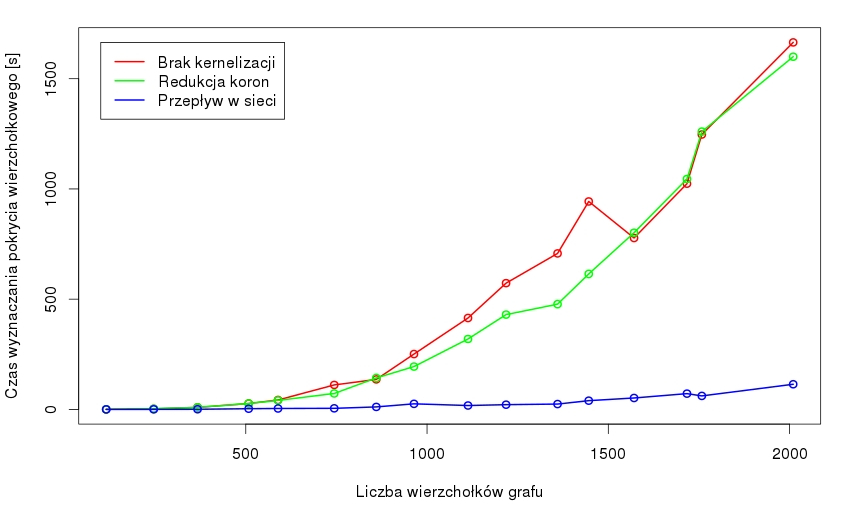
\includegraphics[width=\textwidth]{results-naive}
  \end{figure}
}
\subsubsection{\textbf{Czas wyznaczania pokrycia wierzchołkowego bez przetwarzania wstępnego}}\label{time_vc}
\par{
  Porównanie czasów wyznaczania pokrycia wierzchołkowego bez uprzedniego zastosowania technik przetwarzania wstępnego przedstawia Rysunek~\ref{fig_results_vc}.
  \begin{figure}
    \caption{Czas wyznaczania pokrycia wierzchołkowego bez przetwarzania wstępnego.}
    \label{fig_results_vc}
    \centering
      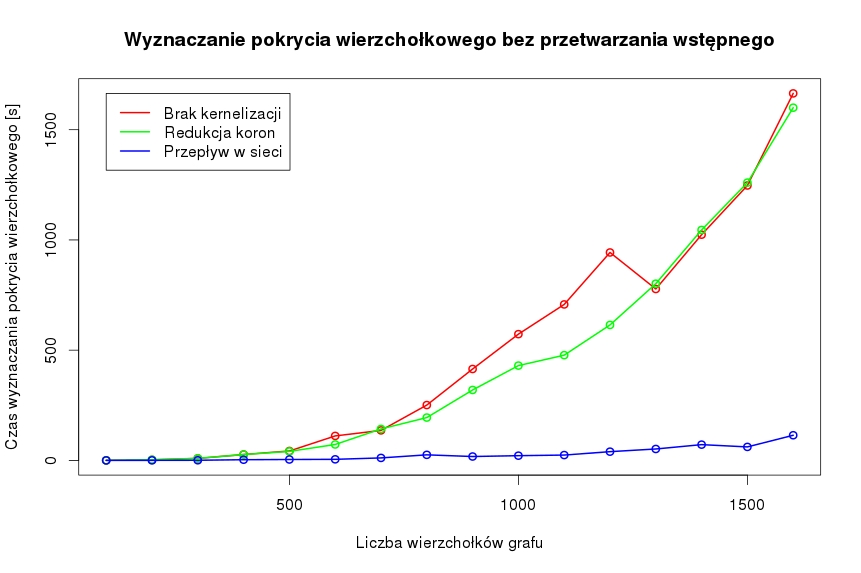
\includegraphics[width=\textwidth]{results-vc}
  \end{figure}
  Wyraźnie widoczny jest pozytywny wpływ zastosowania redukcji dziedziny do jądra problemu przez rozwiązanie przeformułowania problemu do egzemplarza problemu przeływu w sieci.
  Jako prawdopodobne uzasadnienie tego, że redukcja koron nie oferuje tak dużego przyspieszenia jak technika oparta na przepływie w sieci uznano dwa powody.
  \begin{itemize}
    \item Grafy stanowiące dane testowe są ubogie w korony.
    Wynika to z postaci funkcji określającej współczynnik selektywności wierzchołków --- struktury koron wymagają bardzo specyficznych relacji zachodzących pomiędzy zbiorami wierzchołków, mianowicie istnienia zbiorów niezależnych o połączonym sąsiedztwie.
    W ramach procesu przygotowywania danych testowych udało się uzyskać grafy, dla których redukcja dziedziny uzyskana przez usunięcie koron była znacznie większa, jednak grafy te nie pozwalały na uzyskanie wyników dających przedstawić się w postaci funkcji zachowującej choćby pozory monotoniczności.
    \item Zaimplementowana technika wyznaczania koron w grafie oparta jest na zbyt restrykcyjnym uściśleniu NT--redukcji do serii operacji działających bezpośrednio na konkretnych egzemplarzach skojarzeń.
    Najprawdopodobniej stanowi to również powód opisanych w podrozdziale~\ref{sss_problems_ckx} problemów napotkanych przy implementacji algorytmu Chen, Kanj, Xia.
    Pozostałe zaimplementowane egzemplarze NT--redukcji wyznaczają podzbiory różniące się od tych uzyskiwanych przez redukcję proponowaną w pracy~\cite{KernelizationAlgorithms04}.
    Dalsze pole do badań może stanowić weryfikacja czy bardziej ogólne postacie NT--redukcji --- wykonywane za pomocą algorytmów programowania liniowego --- zapewnią lepsze rezultaty dla grafów o strukturze zbliżonej do tych, które wykorzystano jako dane testowe.
  \end{itemize}

  Ze względu na niedoskonałości implementacji opisywanych w niniejszej pracy nie udało się wykonać pomiarów czasu wyznaczania pokrycia wierzchołkowego bez przetwarzania wstępnego dla grafów zawierających więcej niż 1600 wierzchołków.
  Pomimo nieco gorszych od oczekiwanych rezultatów należy zauważyć, że każda z przedstawionych charakterystyk jest o wiele rzędów wielkości lepsza niż charakterystyka uzyskana z pomiarów czasu działania metody siłowej.
}
\subsubsection{\textbf{Czas wyznaczania pokrycia wierzchołkowego po przetwarzaniu wstępnym}}
\par{
  Porównanie czasów wyznaczania pokrycia wierzchołkowego po uprzednim zastosowaniu technik przetwarzania wstępnego przedstawia Rysunek~\ref{fig_results_vc_p}.
  \begin{figure}
    \caption{Czas wyznaczania pokrycia wierzchołkowego po przetwarzaniu wstępnym.}
    \label{fig_results_vc_p}
    \centering
      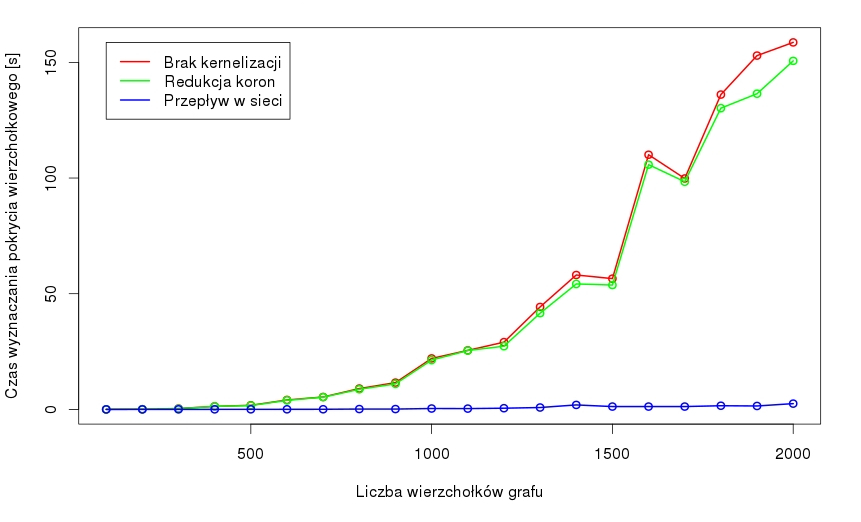
\includegraphics[width=\textwidth]{results-vc-p}
  \end{figure}
  Zastosowanie prostych technik przetwarzania wstępnego opisanych w podrozdziale~\ref{Section_preprocessing} pozwala na dodatkowe skrócenie czasu wyznaczania pokrycia wierzchołkowego w grafach testowych o około dwa rzędy wielkości.
}
\par{
  Ponieważ różnica w czasie wyznaczania pokrycia wierzchołkowego z zastosowaniem techniki opartej o przepływ w sieci pomiędzy wariantem bez przetwarzania wstępnego a wariantem z zastosowaniem przetwarzania wstępnego jest słabo widoczna, Rysunek~\ref{fig_nf_comp} zestawia charakterystyki czasowe tych przypadków.
  \begin{figure}
    \caption{Wpływ przetwarzania wstępnego na czas wyznaczania pokrycia wierzchołkowego w oparciu o przepływ w sieci.}
    \label{fig_nf_comp}
    \centering
      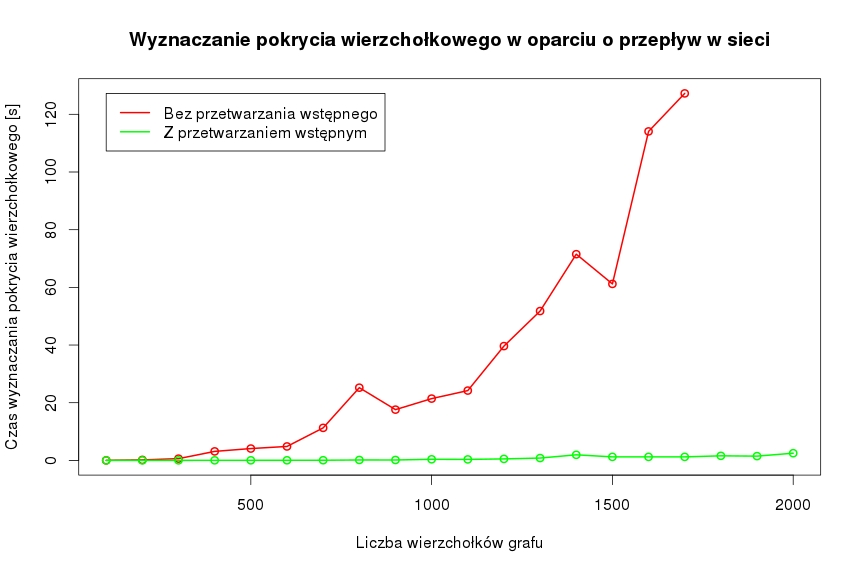
\includegraphics[width=\textwidth]{nf-comp}
  \end{figure}
}
\subsection{Algorytmy przetwarzania wstępnego i redukcji dziedziny do jądra problemu}
\par{
  Redukcja dziedziny do jądra problemu w praktyce może mieć sens jedynie wtedy, gdy czas potrzebny wykonanie operacji zawężających przestrzeń poszukiwań pokrycia wierzchołkowego jest wielomianowy.
  W celu weryfikacji szybkości działania implementacji opisywanych technik redukcji dziedziny oraz przetwarzania wstępnego zmierzono czas potrzebny na wykonanie tych operacji dla zbioru grafów testowych. 
}
\subsubsection{\textbf{Algorytmy redukcji dziedziny do jądra problemu}}
\par{
  Porównanie czasów wyznaczania pokrycia wierzchołkowego bez uprzedniego zastosowania technik przetwarzania wstępnego przedstawia Rysunek~\ref{fig_results_k}.
  \begin{figure}
    \caption{Czas redukcji dziedziny bez przetwarzania wstępnego.}
    \label{fig_results_k}
    \centering
      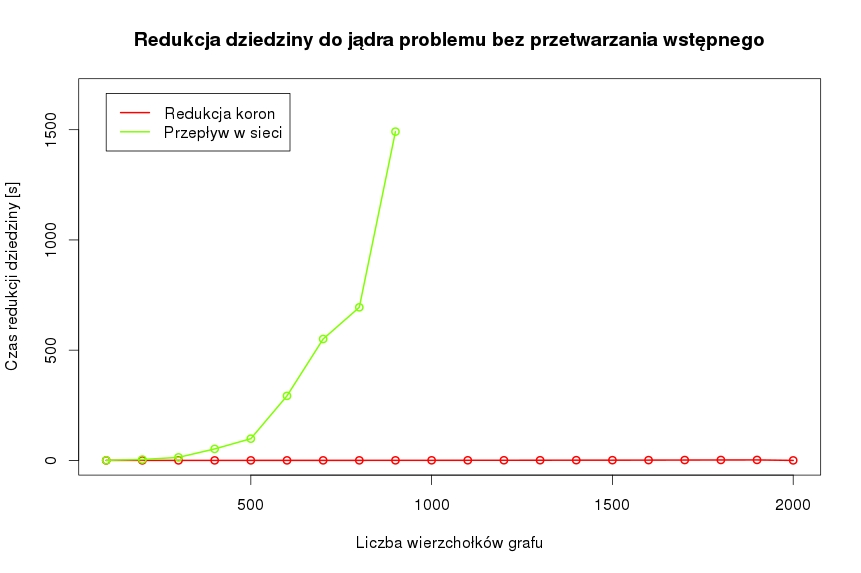
\includegraphics[width=\textwidth]{results-k}
  \end{figure}
  Powodem bardzo niekorzystnej złożoności czasowej działania algorytmu redukcji dziedziny przez rozwiązanie przeformułowania problemu do egzemplarza problemu przepływu w sieci są błędy popełnione przy implementacji koncepcji opisanej w pracy~\cite{KernelizationAlgorithms04}.
  Szczegóły tych błędów oraz proponowane usprawnienia opisane są w podrozdziale~\ref{s_improvements}.
  Ponieważ charakterystyka wyników pomiarów czasu działania tego algorytmu jest zdeformowana i nie ukazuje prawdziwej jego szybkości, a także ze względu na bardzo długi czas oczekiwania, ograniczono dziedzinę przetwarzanych przez niego grafów do zawierających najmniejszą liczbę wierzchołków.
  W związku z zaciemnieniem na wykresie wartości wyników pomiarów czasu działania algorytmu redukcji koron, Rysunek~\ref{fig_results_k_crown} przedstawia wyłącznie tę charakterystykę.
  \begin{figure}
    \caption{Czas redukcji dziedziny przez wyznaczenie i usunięcie koron bez przetwarzania wstępnego.}
    \label{fig_results_k_crown}
    \centering
      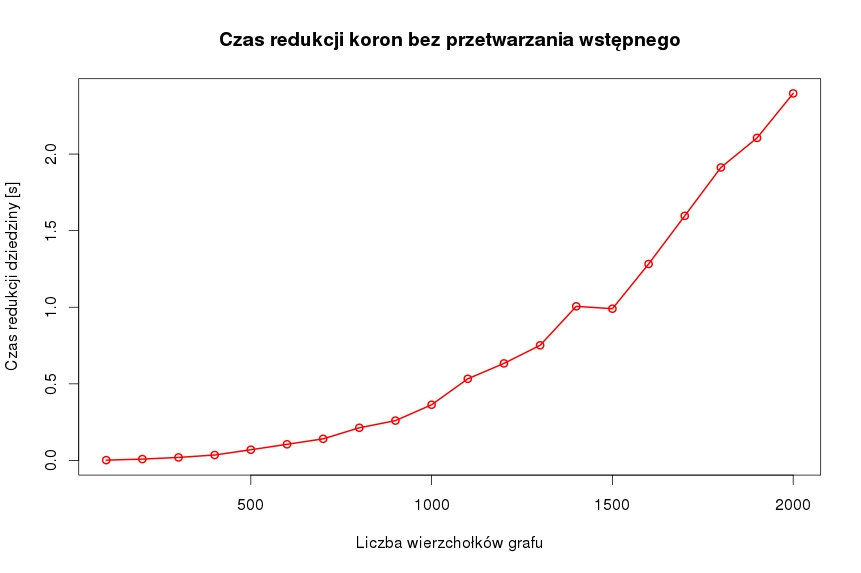
\includegraphics[width=\textwidth]{results-k-crown}
  \end{figure}
}
\par{
  Na Rysunku~\ref{fig_results_k_crown} można zauważyć gwałtowny spadek czasu działania algorytmu redukcji koron dla grafu o dwóch tysiącach wierzchołków.
  Jest on spowodowany napotkaniem przez algorytm sytuacji świadczącej o tym, że w grafie nie może istnieć korona --- prowadzi to do natychmiastowego zakończenia jego działania.
  Biorąc pod uwagę to, że zbiór grafów testowych jest efektem wielu prób przygotowania odpowiedniego zestawu danych przy doborze różnych parametrów generacji grafów, ten przypadek uświadamia jak bardzo wrażliwy na strukturę grafu jest algorytm redukcji koron.
}
\par{
  Rysunek~\ref{fig_results_k_crown_p} przedstawia wpływ uprzedniego zastosowania algorytmów przetwarzania wstępnego na czas działania algorytmu redukcji koron.
  \begin{figure}
    \caption{Czas redukcji dziedziny bez przetwarzania wstępnego.}
    \label{fig_results_k_crown_p}
    \centering
      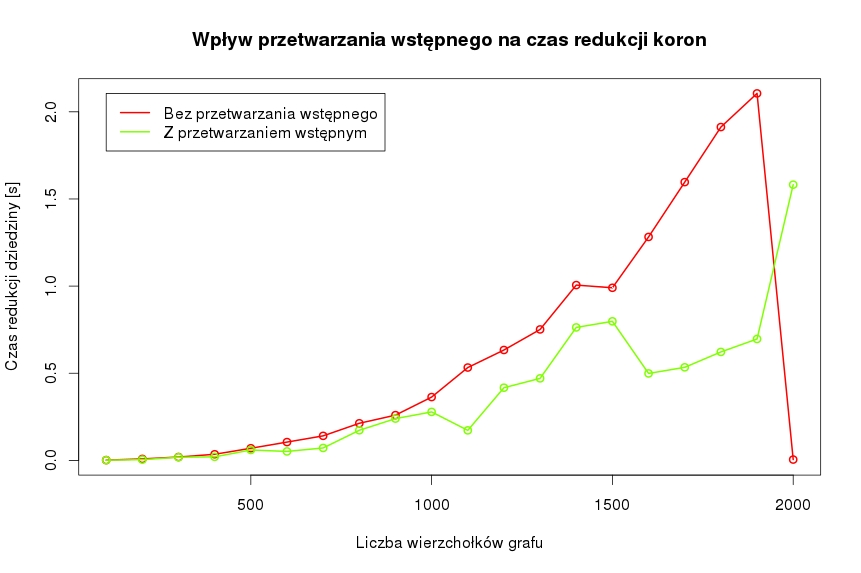
\includegraphics[width=\textwidth]{results-k-crown-p}
  \end{figure}
  Oprócz poprawy czasu działania procedury redukcji koron widać tutaj pewną zmianę w kontekście operacji na największym grafie.
  Ponieważ algorytm przetwarzania wstępnego zmienia strukturę grafu wejściowego, może prowadzić on do pojawienia się w dziedzinie struktur nie istniejących w nim wcześniej.
  Na podstawie Rysunku~\ref{fig_results_k_crown_p} można domniemać, że zwinięcie pewnego połączonego sąsiedztwa wierzchołka $v$ stopnia $d(v)=2$ w grafie wejściowym lub usunięcie pewnego wierzchołka $u$ spełniającego kryteria opisane w podrozdziale~\ref{Section_preprocessing} spowodowało pojawienie się w grafie zbiorów wierzchołków $I, H$ spełniających własności pozwalające włączyć je do korony.
  W tym wypadku przetwarzanie wstępne otwarło drogę do dodatkowej redukcji dziedziny w dalszych etapach.\footnote{Nawiązując do opisanych w podrozdziale~\ref{time_vc} problemów należy również brać pod uwagę to, że bardziej ogólna implementacja procedury redukcji korony może być w stanie wykryć rzeczone struktury nawet bez przetwarzania wstępnego dzięki algorytmowi programowania liniowego.}
}
\par{
  Rysunek~\ref{fig_results_p} przedstawia charakterystykę czasu przetwarzania wstępnego w zależności od liczby wierzchołków grafu.
  \begin{figure}
    \caption{Czas przetwarzania wstępnego.}
    \label{fig_results_p}
    \centering
      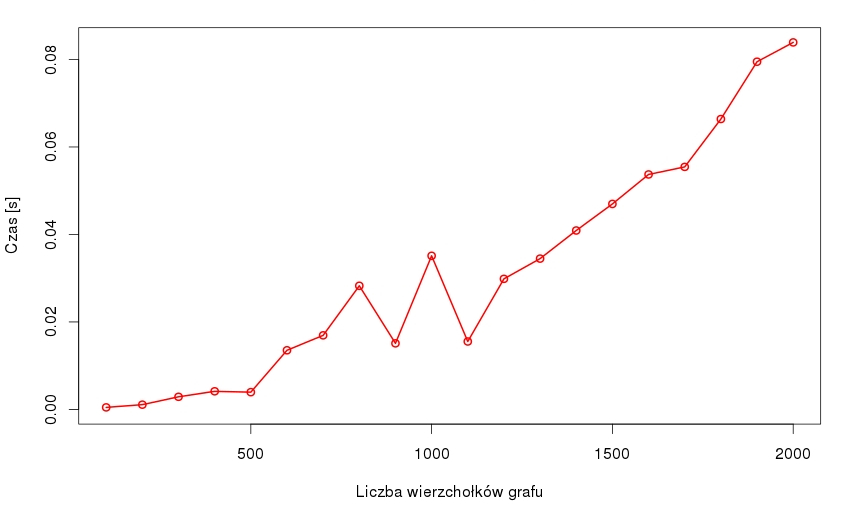
\includegraphics[width=\textwidth]{results-p}
  \end{figure}
}
\section{Wnioski}

  \chapter{Podsumowanie i~kierunki dalszych prac}
\label{summary}
\section*{Proponowane usprawnienia i~kierunki rozwoju}\label{s_improvements}
\addtocounter{section}{1}
  \subsubsection{\textbf{Pełna implementacja algorytmu Chena, Kanji oraz Xia.}}\label{sss_problems_ckx}

  Ze względu na wysoką złożoność analityczną algorytmu Chena, Kanji oraz Xia nie udało się zaimplementować wszystkich elementów składowych wymaganych przez główny algorytm w~stopniu pozwalającym na przeprowadzenie badań eksperymentalnych z~jego wykorzystaniem.
  Głównym problemem był dobór NT--dekompozycji, którą posługuje się funkcja \textsc{Zwijanie}, działająca zgodnie z~pseudokodem~\ref{alg_ckx_gf}.
  Problem ten polegał na zastosowaniu dekompozycji wyznaczającej korony w~grafie, zaimplementowanej zgodnie z~wytycznymi opisywanymi w~pracy~\cite{KernelizationAlgorithms04} i działająca zgodnie z~pseudokodem~\ref{alg_findCrown} w kontekście odszukiwania pseudokoron.
  Proponowane jest zbadanie wpływu innego rodzaju NT--dekompozycji na poprawność działania algorytmu \textsc{Zwijanie}.
  Kod źródłowy zawiera kilka przykładowych implementacji NT--dekompozycji uzyskiwanych w~oparciu na rozwiązaniu sformułowania problemu jako zadania programowania liniowego.

  Usprawnienie logiki związanej z~funkcją \textsc{Zwijanie} spowoduje, że implementacja algorytmu Chena, Kanji oraz Xia będzie bardziej wydajna.
  Dalsze usprawnienia będą dotyczyć części algorytmu zajmującej się utrzymywaniem kolejki priorytetowej struktur, która usuwa krotki o~wartości $q = 0$ oraz wykonuje algorytm siłowy w~sytuacji, gdy algorytm główny dociera do punktu, gdzie zachodzi $k \leq 7$.

  \subsubsection{\textbf{Badania eksperymentalne dla różnych implementacji procedur składowych algorytmu Chena, Kanji oraz Xia pominiętych w~pracy źródłowej.}}

  Omawiany algorytm jest skomplikowany i żmudny w~analizie.
  Duża złożoność esencjonalna problemu prowadzi do zastosowania pewnych skrótów myślowych w~treści pracy~\cite{ImprovedBounds10}.
  Poczynione przez autorów założenia mówiące, że algorytm niejawnie wykonuje pewne operacji znacząco utrudniają implementację, a w~szczególności implementację zoptymalizowaną.
  Operacje te w~praktyce są niebagatelnymi kwestiami i~stanowią pole do dalszych badań i optymalizacji pozwalających na poprawę średniej złożoności obliczeniowej stworzonego rozwiązania.

  \subsubsection{\textbf{Poprawa wydajności czasowej implementacji techniki redukcji dziedziny w~oparciu o~algoretm przepływu w~sieci.}}

  Pozytywny wpływ technik redukcji dziedziny do jądra problemu pokrycia wierzchołkowego jest widoczny i~zaświadcza o~poprawności implementacji.
  Uzyskane wyniki testów wydajnościowych pokazują jednak, że implementacje opisywanych technik zrealizowane w~ramach niniejszej pracy wymagają optymalizacji w~celu uzyskania wydajności bliższej teoretycznej.
  W szczególności implementacja algorytmu redukcji opartej o~przepływ w~sieci boryka się z problemami wydajnościowymi w~związku z~zastosowanym sposobem wyznaczania zbioru $R$, zawierającego wierzchołki osiągalne ze zbioru $S$ przez $M$-przemienne ścieżki.
  Proponowane jest usprawnienie tej części kodu przez zastosowanie odpowiedniego, ogólnie przyjętego za efektywny i~szybki algorytmu pozwalającego określić osiągalność wierzchołka w~grafie począwszy od danego innego wierzchołka.

  \subsubsection{\textbf{Poprawa złożoności pamięciowej.}}

  Cel pracy stanowiła analiza i~implementacja omówionych algorytmów.
  Zaproponowane rozwiązania mogą być zoptymalizowane również w kontekście zużycia pamięci.
  Przedkładając czytelność kodu nad zużycie pamięci, uwagę skupiono na odzwierciedleniu wyników pośrednich w~postaci zmiennych oraz jak najłatwiejszym korzystaniu ze struktur danych, na których opierają się implementowane techniki.
  W załączonej implementacji wszelkie struktury inicjowane są z maksymalną pesymistyczną pojemnością względem analizowanego grafu, nie biorąc pod uwagę na przykład wierzchołków czy krawędzi usuniętych z~grafu.
  Proponowaną optymalizacją jest stworzenie wersji kodu oszczędniej korzystającej ze zmiennych, a także bardziej konserwatywnie rezerwującej potrzebną pamięć.
  Na uwadze warto mieć również wykorzystanie przez język Go mechanizmu odśmiecania pamięci --- implementacje algorytmów muszą być skonstruowane w~sposób sprzyjający jak najszybszym 

  \subsubsection{\textbf{Zbadanie wpływu różnych wariantów NT--dekompozycji na szybkość działania i~efektywność zaimplementowanych algorytmów.}}

  Zastosowane w~niniejszej pracy uściślenie operacji NT--redukcji nie jest oparte bezpośrednio na rozwiązaniu zadania programowania liniowego, lecz na iteracyjnym poruszaniu się po skojarzeniu grafu w~celu wyznaczenia korony.
  Badania eksperymentalne uwidoczniły pewne problemy spowodowane tym podejściem.
  Istnieje potencjał poprawy efektywności algorytmów redukujących dziedzinę w bezpośrednim oparciu na koncepcji NT--dekompozycji.
  W ramach niniejszej pracy zaimplementowano kilka przykładowych NT--dekompozycji (NT--dekompozycja wg. Bar-Yehudy oraz NT--dekompozycja wg. J.F. Bussa).
  Jako kierunek dalszych prac proponowane jest przeprowadzenie badań eksperymentalnych wpływu zastosowania poszczególnych NT--dekompozycji w~algorytmie redukcji koron oraz algorytmie Chena, Kanji oraz Xia na efektywność zawężania dziedziny grafu.

\section*{Podsumowanie i~wnioski}
\addtocounter{section}{1}
  W~ramach niniejszej pracy omówiono oraz zaimplementowano pięć algorytmów służących do redukcji złożoności czasowej rozwiązania problemu pokrycia wierzchołkowego grafu. Przeprowadzono badania szybkości działania dla czterech z~nich.
  Przypadki testowe obejmowały wyznaczanie pokrycia wierzchołkowego i~działanie algorytmów redukcji dziedziny do jądra problemu na niezmodyfikowanym grafie wejściowym oraz na grafie poddanym uprzedniemu wykonaniu algorytmu przetwarzania wstępnego.

  W oparciu o~wyniki badań eksperymentalnych określenie najszybszego spośród zaimplementowanych algorytmów nie jest możliwe.
  Głównym powodem jest skupienie się na poprawności czytelności stworzonych rozwiązań, pozostawiając szybkość i zużycie pamięci na drugim planie, co opisano w~podrozdziale~\ref{s_improvements}.
  Algorytm rozwiązujący przeformułowanie problemu jako zadania przepływu w~sieci wykazuje największą efektywność w redukcji dzedziny --- czas wyznaczania pokrycia wierzchołkowego w~grafie zredukowanym omawianą techniką był najniższy spośród wszystkich metod dla większości przypadków testowych.
  Pomimo koncepcyjnej poprawności i~wysokiej efektywności w~redukcji dziedziny, czas jej działania w~porównaniu do pozostałych metod jest znacznie dłuższy, co oznacza, że stworzone w~ramach niniejszej pracy rozwiązanie nie jest zalecane do użytku praktycznego.
  W przypadku algorytmu redukcji koron, ciężko mówić o uniwersalności tego podejścia.
  Wiąże się to z~uzależnieniem szybkości działania tej metody od bardzo charakterystycznych struktur występujących w~grafie.
  W związku ze sposobem generacji losowych grafów testowych, były one ubogie w~te struktury, co spowodowało spadek efektywności zawężania dziedziny przez algorytm redukcji koron, widoczny na charakterystykach porównujących czas wyznaczania pokrycia wierzchołkowego dla grafu przetworzonego poszczególnymi metodami.

  Mimo napotkanych problemów, drogą analizy i~badań eksperymentalnych udało się wykazać pozytywny wpływ omawianych technik na złożoność czasową rozwiązania problemu pokrycia wierzchołkowego dla grafów ogólnych.

  Oprócz zaproponowanych implementacji, badań oraz~analizy zostały również zaproponowane usprawnienia i~potencjalne rozszerzenia, które zwiększą jakość oraz poprawią wydajność omawianych metod.
  Interesujące z~perspektywy dalszych badań jest zastosowanie innych wariantów koncepcji wykorzystywanych przez zaimplementowane algorytmy --- takich jak NT--dekompozycja --- w celu zbadania wpływu ich zmiany na złożoność czasową algorytmów oraz ich efektywność w redukcji dziedziny grafu.

  \addcontentsline{toc}{chapter}{\bibname}
  \bibliography{Main}

  % \renewcommand{\appendixname}{Dodatek}

  \end{document}
